\documentclass[a4paper,12pt]{book}

\usepackage[left=2.25cm,right=2.25cm,top=2.5cm,bottom=2.5cm]{geometry}
\usepackage[T1]{fontenc}
\usepackage[utf8]{inputenc}
\usepackage[spanish]{babel}
\usepackage{graphicx}
\usepackage{subcaption}
\usepackage{listings}
\usepackage{color}
\usepackage{colortbl}
% Alternativas de fncychap: Sonny, Lenny, Glenn, Conny, Rejne, Bjarne.
\usepackage[Rejne]{fncychap}
\usepackage{type1cm} % scalable fonts
\usepackage{lettrine}
\usepackage{fancyhdr}
\usepackage{moreverb}
% Identacion y separacion de parrafos
\usepackage{parskip}
% Posicion de figuras
\usepackage{float}
% Diagramas
\usepackage{pstricks, pst-node, pst-tree}
\usepackage{xyling}
% Tablas
\usepackage{multirow}
% Ejemplos y definiciones
\usepackage{amsthm}
% Mejor que eqnarray : align
\usepackage{amsmath}
% Símbolos AMS
\usepackage{amssymb}
% Tablas con líneas de puntos
\usepackage{array}
\usepackage{arydshln}
% Dos columnas
\usepackage{multicol}
% Diagramas de autómatas
\usepackage{gastex}
% Tabla de contenidos por capítulo
%\usepackage[spanish]{minitoc}
% Hiperenlaces
\usepackage[bookmarks]{hyperref}
\hypersetup{
    colorlinks,
    citecolor=black,
    filecolor=black,
    linkcolor=black,
    urlcolor=black,
	linktocpage
}
\renewcommand{\rmdefault}{ptm}

\begin{document}
\nocite{*}
\title{Python}
\author{Eduardo Martínez Graciá, Mercedes Valdés Vela, Santiago Paredes Moreno, José Manuel Juárez Herrero}

\renewcommand{\tablename}{Tabla}
\newcommand{\HRule}{\rule{\linewidth}{0.5mm}}
\renewcommand{\chaptermark}[1]{\lhead[{\sc{\chaptername\ #1}}]{}}
\renewcommand{\sectionmark}[1]{\rhead[ ]{{\thesection.\ #1}}}


\begin{titlepage}

\begin{center}

% Upper part of the page
\vfill

\includegraphics[height=0.18\textwidth]{imagenes/FIUM}\\[2.5cm]

\textsc{\LARGE Autómatas y Lenguajes Formales}\\[0.5cm]

\textsc{\Large Grado en Ingeniería Informática}\\[0.5cm]


% Title
\HRule \\[0.4cm]
{ \huge \bfseries Apuntes de Python}\\[0.4cm]

\HRule \\[1.5cm]

% Author and supervisor
\begin{minipage}{0.5\textwidth}
\begin{center}
\large
\emph{Autores:}\\
Eduardo \textsc{Martínez Graciá}\\
edumart@um.es\\
Mercedes \textsc{Valdés Vela}\\
mdvaldes@um.es\\
Santiago \textsc{Paredes Moreno}\\
chapu@um.es\\
José Manuel \textsc{Juárez Herrero}\\
jmjuarez@um.es
\end{center}
\end{minipage}

\vskip 2em

\includegraphics[height=0.18\textwidth]{imagenes/Python-logo}

\vfill

% Bottom of the page
{\large \today}

\end{center}

\end{titlepage}

\clearpage

\pagestyle{empty}

\null \vfill

\clearpage{\pagestyle{empty}\cleardoublepage}

\setcounter{page}1
\setcounter{secnumdepth}{4}	%Profundidad de la numeracion del indice
\setcounter{tocdepth}{2}	%Profundidad del indice

%\dominitoc
%\faketableofcontents

\pagestyle{fancy}
\renewcommand{\chaptername}{}
\renewcommand{\chaptermark}[1]{\lhead[{\sc{\chaptername\ \thechapter.\ #1}}]{}}
\renewcommand{\sectionmark}[1]{\rhead[ ]{{\thesection.\ #1}}}
\renewcommand{\headrulewidth}{0.5pt}
\renewcommand{\footrulewidth}{0.5pt}
\setlength{\headheight}{14pt}

\lstset{
    breaklines=true,
    %
    extendedchars=true,
    literate=
	{¿}{{?`}}1 {¡}{{!`}}1
    {á}{{\'a}}1 {é}{{\'e}}1 {í}{{\'i}}1 {ó}{{\'o}}1 {ú}{{\'u}}1
    {Á}{{\'A}}1 {É}{{\'E}}1 {Í}{{\'I}}1 {Ó}{{\'O}}1 {Ú}{{\'U}}1
    {à}{{\`a}}1 {è}{{\`e}}1 {ì}{{\`i}}1 {ò}{{\`o}}1 {ù}{{\`u}}1
    {À}{{\`A}}1 {È}{{\'E}}1 {Ì}{{\`I}}1 {Ò}{{\`O}}1 {Ù}{{\`U}}1
    {ä}{{\"a}}1 {ë}{{\"e}}1 {ï}{{\"i}}1 {ö}{{\"o}}1 {ü}{{\"u}}1
    {Ä}{{\"A}}1 {Ë}{{\"E}}1 {Ï}{{\"I}}1 {Ö}{{\"O}}1 {Ü}{{\"U}}1
    {â}{{\^a}}1 {ê}{{\^e}}1 {î}{{\^i}}1 {ô}{{\^o}}1 {û}{{\^u}}1
    {Â}{{\^A}}1 {Ê}{{\^E}}1 {Î}{{\^I}}1 {Ô}{{\^O}}1 {Û}{{\^U}}1
    {œ}{{\oe}}1 {Œ}{{\OE}}1 {æ}{{\ae}}1 {Æ}{{\AE}}1 {ß}{{\ss}}1
    {ç}{{\c c}}1 {Ç}{{\c C}}1 {ø}{{\o}}1 {å}{{\r a}}1 {Å}{{\r A}}1
    {€}{{\EUR}}1 {£}{{\pounds}}1 {ñ}{{\~n}}1 {Ñ}{{\~N}}1 
}

\setlength{\parindent}{15pt}
\setlength{\itemindent}{15pt}

\lstset{basicstyle=\fontsize{12}{13}\ttfamily,showstringspaces=false,language=Python,numbers=left,numberstyle=\tiny,frame=tb,columns=fullflexible,inputencoding=utf8}

\clearpage{\pagestyle{empty}\cleardoublepage}

\pagestyle{plain}

\section*{Agradecimientos}

El uso de Python en las prácticas de Autómatas y Lenguajes Formales se podría haber quedado en un simple proyecto si no hubiésemos contado con la ayuda de un alumno interno con suficiente entusiasmo como para iniciar el camino. Adrián Cánovas Rodríguez colaboró con los profesores de la asignatura durante el curso 2017/2018, probando las posibilidades del lenguaje para ser empleado en el desarrollo del tipo de aplicaciones que se plantean en los enunciados de prácticas. Elaboró una primera versión del manual de instalación de Eclipse con Python, así como el código para cargar y manejar desde Python los autómatas finitos deterministas generados con las versiones 7 y 8-beta de la herramienta JFLAP.

\clearpage{\pagestyle{empty}\cleardoublepage}

\setcounter{page}1
\setcounter{secnumdepth}{4}	%Profundidad de la numeracion del indice
\setcounter{tocdepth}{2}	%Profundidad del indice

\tableofcontents
\clearpage{\pagestyle{empty}\cleardoublepage}

\pagestyle{fancy}

% Capítulo 1: Introducción
%!TEX root = Python.tex

\chapter{Introducción}

\lettrine[lines=5]{A}{} partir del curso 2018/2019, la asignatura de Autómatas y Lenguajes Formales comienza a emplear Python en las prácticas de programación. Emplear este lenguaje conlleva algunas ventajas con respecto a su predecesor, Java. En primer lugar, el lenguaje Python se concibió para que fuese fácil de aprender. En las primeras semanas del curso se impartirán seminarios sobre este lenguaje que darán las bases para desarrollar aplicaciones de validación de cadenas con autómatas finitos y expresiones regulares, y de traducción entre formatos de ficheros. Además, Python es un lenguaje en continua expansión, cada vez más usado en sectores con una fuerte proyección de futuro, como el análisis de datos, el cálculo científico y la bioinformática. Creemos que el hecho de usar uno de los lenguajes más populares en la actualidad puede dar una mayor motivación para abordar las prácticas de la asignatura.

Es necesario realizar una \emph{advertencia} antes de seguir: estos apuntes no son un manual del lenguaje Python. Únicamente pretenden recoger lo que es necesario para abordar los problemas tratados en la asignatura. Además, están enfocados a alumnos que tienen cierto conocimiento del lenguaje C, ya que en numerosas ocasiones se compara la forma de realizar algo en este lenguaje y en Python. Para un estudio más amplio de Python, se recomienda la consulta de las referencias bibliográficas que aparecen al final de estos apuntes.

\section{Breve historia de Python}

El lenguaje Python fue concebido inicialmente por el informático holandés Guido Van Rossum, cuando trabajaba en el \emph{Centrum Wiskunde \& Informatica}\footnote{Centro para las Matemáticas y la Ciencia de la Computación (\url{http://www.cwi.nl}).} (CWI) de Ámsterdam hacia finales de los ochenta. Van Rossum formaba parte del equipo dedicado al desarrollo del sistema operativo distribuido \emph{Amoeba} (proyecto liderado por Andrew Tanenbaum), y su objetivo al crear Python era proporcionar un lenguaje de programación que pudiese cubrir el hueco que existía en Amoeba entre el lenguaje C y el shell del sistema. Hacía falta un lenguaje de alto nivel con mayor potencia expresiva que el shell pero sin las dificultades de C, que en Amoeba tenía un interfaz de programación con el sistema bastante complicado. 

Según el propio Van Rossum\footnote{En el blog de Guido Van Rossum sobre la historia de Python (http://python-history.blogspot.com), se puede leer lo siguiente: \emph{I picked the first thing that came to mind, which happened to be Monthy Python’s Flying Circus, one of my favorite comedy troupes. The reference felt suitably irreverent for what was essentially a “skunkworks project”. The word “Python” was also catchy, a bit edgy, and at the same time, it fit in the tradition of naming languages after famous people, like Pascal, Ada, and Eiffel. The Monty Python team may not be famous for their advancement of science or technology, but they are certainly a geek favorite. It also fit in with a tradition in the CWI Amoeba group to name programs after TV shows.}}, el nombre del lenguaje es un homenaje a los cómicos ingleses Monty Python. Existen lenguajes cuyos nombres proceden de personajes famosos, como Pascal, Ada o Eiffel. Python sería, salvando las distancias, una continuación de esta tradición. 

\begin{figure}
\captionsetup[subfigure]{labelformat=empty}
\begin{subfigure}{0.48\textwidth}
\includegraphics[width=\linewidth]{imagenes/Guido-van-Rossum}
\caption{Guido Van Rossum} \label{fig:guido-van-rossum}
\end{subfigure}
\hspace*{\fill} 
\begin{subfigure}{0.48\textwidth}
\includegraphics[width=\linewidth]{imagenes/Monty-Python}
\caption{Monty Python} \label{fig:monty-python}
\end{subfigure}
\caption{Personajes relevantes en el origen de Python}
\end{figure}

Una de las fuentes de inspiración de Van Rossum para la concepción de Python fue el lenguaje \emph{ABC}, también desarrollado en el CWI de Ámsterdam, que pretendía ser un sustituto del lenguaje \emph{BASIC} (aparecido hacia los sesenta) para la enseñanza de la programación. Python tiene una sintaxis en la que la sencillez es un principio esencial para atraer a programadores noveles, pero también asume algunas notaciones sintácticas propias de lenguajes con mucha implantación, como C, para que los programadores experimentados puedan usar Python con facilidad.

La primera versión pública de Python se presenta en 1991. El año 1996, Van Rossum continúa desarrollando el lenguaje con un equipo de colaboradores en el \emph{Corporation for National Research Institute} (CNRI) en Reston, Virginia (EE.UU.), una organización sin ánimo de lucro cuyo objetivo es la promoción de las tecnologías de la información. En colaboración con la agencia estatal estadounidense \emph{Defense Advanced Research Projects Agency} (DARPA), el año 1999 se inicia un proyecto para estudiar la aplicación de Python a la enseñanza de la programación. En el año 2001 se creó la \emph{Python Software Foundation} (PSF)\footnote{Web de la fundación: \url{https://www.python.org/psf-landing/}.}, siguiendo el modelo de la fundación Apache\footnote{Fundación sin ánimo de lucro dedicada al desarrollo de aplicaciones gratuitas, empezando por el famoso servidor HTTP: \url{https://www.apache.org/}.}, y se lanzó la versión 2.1 del lenguaje que contaba con una licencia compatible con la \emph{General Public Licence} de GNU. De 2005 a 2012 Van Rossum pasa a trabajar en Google, y de 2013 a la actualidad en Dropbox, potenciando a través de estas compañías la divulgación y el uso del lenguaje Python.

Van Rossum ha sido el \emph{Benevolent Dictator for Life} (BDFL)\footnote{Dictador benevolente vitalicio.} en la comunidad de desarrolladores de Python, es decir, ha asumido la responsabilidad de tomar las decisiones finales sobre la evolución del lenguaje. Su \emph{benevolente dictadura} se ha caracterizado por una actitud conservadora, admitiendo pocos cambios al lenguaje entre versiones sucesivas. Sin embargo, no han sido nada \emph{benevolentes} las fuertes críticas que ha recibido por adoptar esta postura, hasta el punto de que, el 12 de julio de 2018, con un mensaje enviado a la lista de python-committers\footnote{En \url{https://www.mail-archive.com/python-committers@python.org/msg05628.html} se puede leer el mensaje de retirada de Guido Van Rossum. La revolución en la comunidad de Python se ha desencadenado a raíz de una acalorada discusión en torno a permitir o no el uso de asignaciones en expresiones. Se puede consultar en el Python Enhancement Proposal (PEP) 572: \url{https://www.python.org/dev/peps/pep-0572/}. Y es que, por lo que parece, la sintaxis de los lenguajes de programación desata pasiones.}, anunció su completa retirada de la toma de decisiones sobre la evolución del lenguaje. No ha nombrado a ningún sucesor, de modo que todo apunta a que se va a formar un grupo de expertos entre los desarrolladores de Python más destacados, que adoptarán las decisiones estratégicas por votación.


\section{Características principales}

Python es un lenguaje de programación cuyo uso combina un compilador y un intérprete, de forma muy similar a Java. El código de los ficheros fuente de Python, con extensión \texttt{.py}, pasa en primer lugar por un compilador, que traduce el programa desde el lenguaje Python a una versión equivalente en un lenguaje de bajo nivel, el llamado \emph{bytecode} de Python (un ensamblador de una máquina virtual). El compilador genera un fichero con extensión \texttt{.pyc} con el mismo nombre que el fichero fuente, compilando sólo los ficheros que han sido modificados.

Una vez que están todos los ficheros fuente del programa compilados, se lanza el intérprete de Python para ejecutar el programa. El intérprete tiene una concepción similar a la de la máquina virtual de Java. Carga y ejecuta los bytecodes, permitiendo que cualquier programa Python se ejecute en cualquier sistema para el cual exista un intérprete. Esto facilita la portabilidad del código Python. Tanto el compilador de referencia (\texttt{CPython}) como el intérprete de Python están escritos en el lenguaje C, garantizando de esta forma una ejecución rápida de ambos.

Aunque no es habitual en el desarrollo de aplicaciones, se puede usar el intérprete de Python interactivamente desde una consola que permite ejecutar directamente operaciones del lenguaje. Este modo de uso de Python sería equivalente al de un shell del sistema operativo, y podría emplearse para ejecutar secuencias de comandos de un solo uso. También podría permitir hacer pequeñas pruebas de código antes de integrarlo en un fichero \texttt{.py}.

Python permite desarrollar aplicaciones usando varios paradigmas de programación. El lenguaje es orientado a objetos, pero se puede usar en gran medida como lenguaje imperativo. Además, es un lenguaje dinámicamente tipado. Esto significa que no es necesario declarar las variables antes de su uso, y que a una misma variable se le pueden asignar valores de tipos de dato distintos a lo largo de la ejecución del programa. La verificación del uso correcto de los tipos en cada operación que use una variable se realiza en tiempo de ejecución.

Otra característica de Python es el manejo autómatico de la memoria. El programador no debe preocuparse de llamar a funciones que reservan o liberan memoria, evitando el manejo de punteros como en C. Además, Python incluye una librería estándar que permite realizar operaciones de gran utilidad: validación y búsqueda de cadenas con expresiones regulares, consultas sobre ficheros XML, programación de aplicaciones que usan protocolos de red como HTTP, y un largo etcétera. Por esta razón, Python es una opción muy interesante para implementar prototipos de aplicaciones de forma rápida.


\section{Entorno de desarrollo}

En esta sección se indican los pasos necesarios para disponer de una versión actualizada del compilador e intérprete de Python, integrada en la herramienta de desarrollo Eclipse, con el fin de disponer de un entorno de desarrollo similar al que está instalado en los laboratorios de la FIUM.

\subsection{Instalación de Python}\label{sec:instalacion}

En primer lugar, es necesario descargar e instalar la última versión de Python 3 en nuestro equipo. En el momento de escribir este manual, está disponible la versión 3.7.0\footnote{Resultar curioso que exista una versión 2.7.15 también reciente. Esto es así porque, en realidad, hay dos ramas de desarrollo de Python, pero nosotros emplearemos la versión 3.7.0.}.

En función del sistema que estemos empleando, tenemos dos opciones para hacer la instalación. Si usamos Windows o Mac OS X, podemos descargar el instalador que necesitemos, y si usamos alguna distribución de Linux, será más sencillo emplear el comando adecuado para la instalación de software en el sistema, como \texttt{apg-get} o \texttt{yum}. Lo vemos en detalle en las siguientes secciones.

\subsubsection{Windows}

Descarga desde \url{https://www.python.org/downloads/release/python-370/} el instalador adecuado a tu Windows (figura \ref{fig:instalacion}). De las tres opciones disponibles para sistemas de 64 bits (x86-64) o de 32 bits (x86), la que termina con la denominación \emph{executable installer} contiene todo lo necesario para realizar la instalación sin necesidad de tener conexión a Internet en el equipo. Otra opción es usar la que termina con \emph{web-based installer}, que permite indicar durante la instalación qué partes del lenguaje queremos instalar, y requiere conexión a Internet para descargar los ficheros necesarios. La opción tercera, \emph{embeddable zip file}, se emplea cuando hace falta incluir en una aplicación un intérprete de Python 3.7.0. No usaremos esta última opción.

Cuando ejecutes el instalador, es importante que marques la opción que indica \emph{Add Python 3.7 to PATH}, para que se pueda invocar a Python desde línea de comandos (figura \ref{fig:windows}).

\begin{figure}
\begin{center}
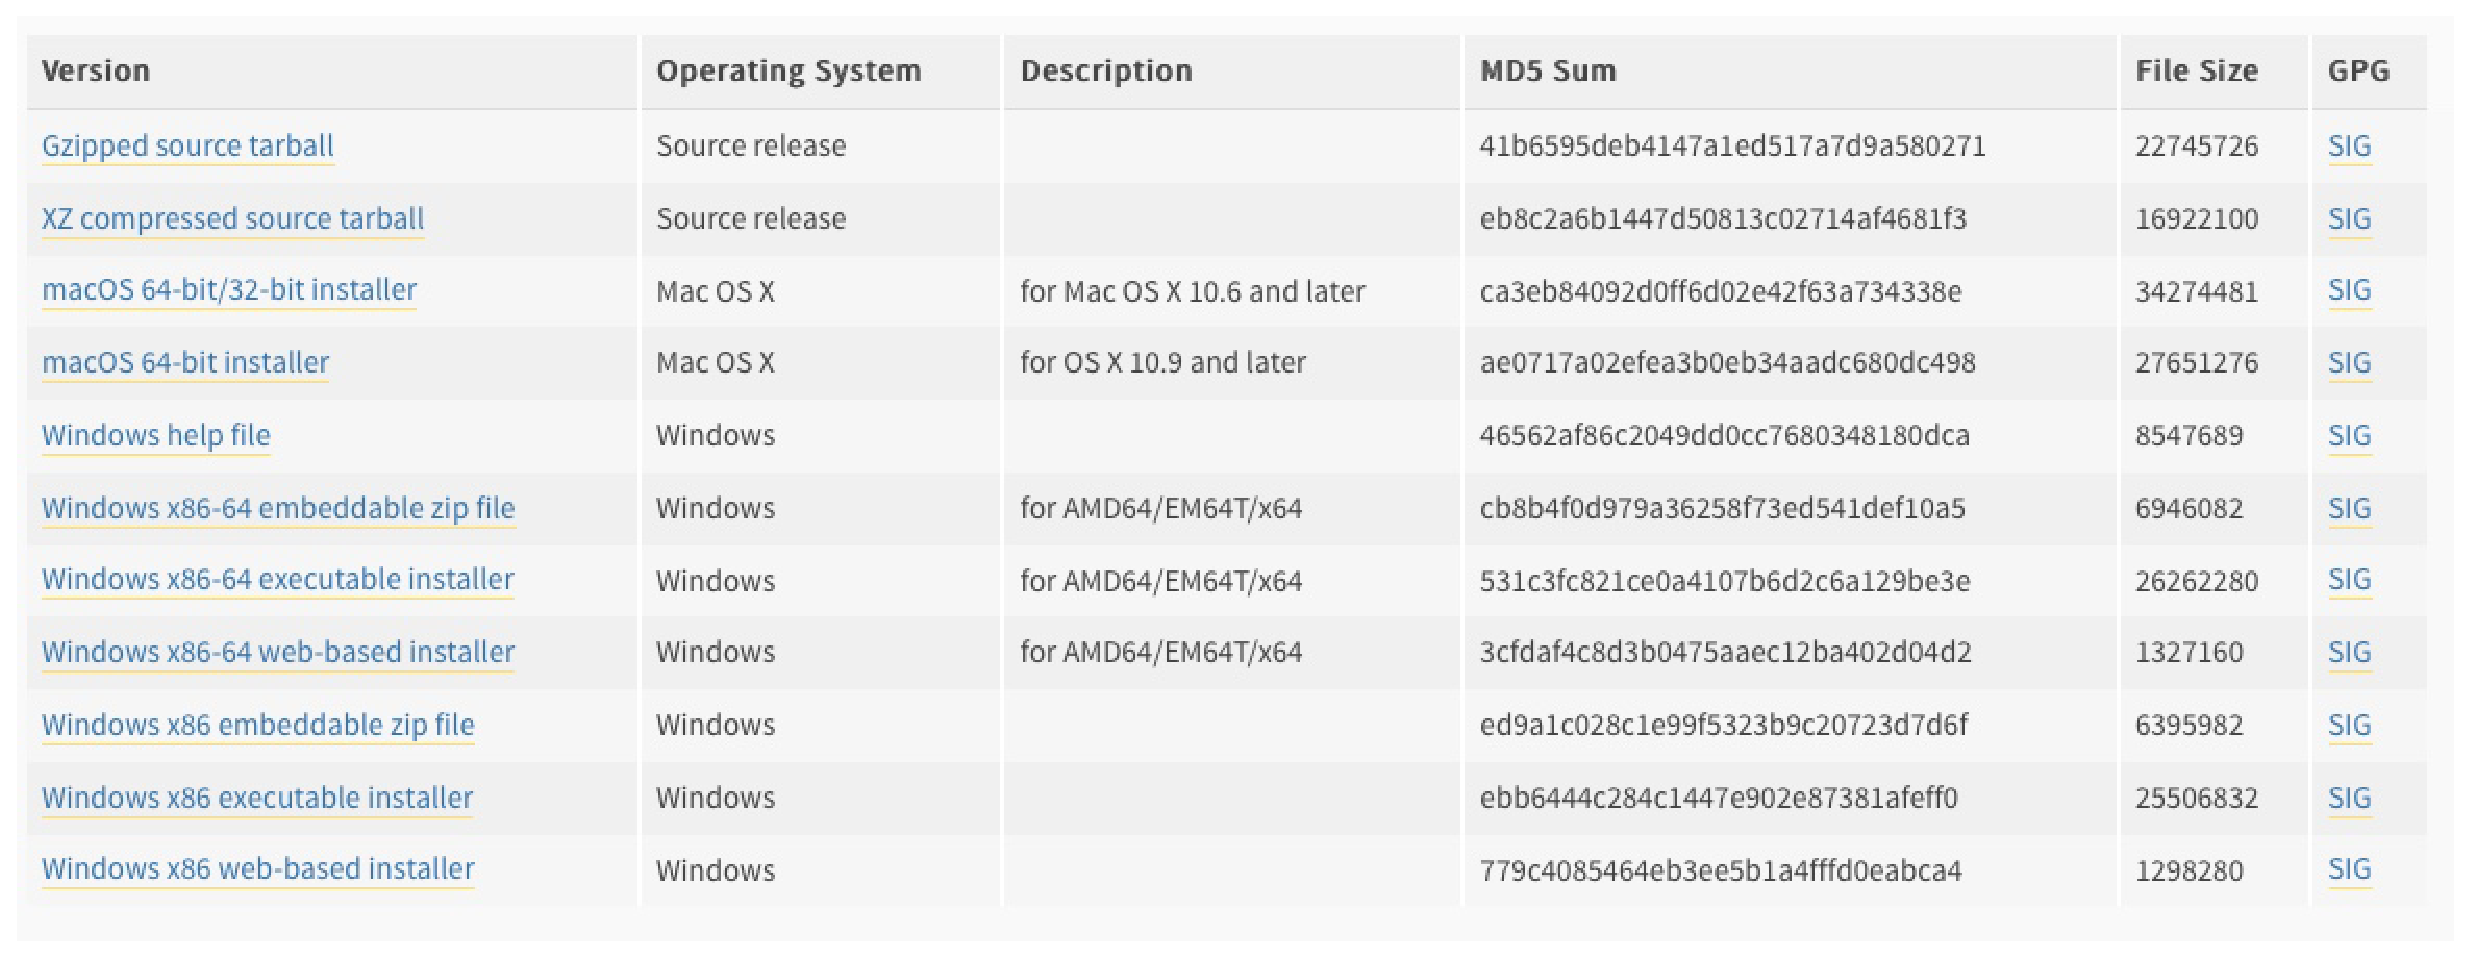
\includegraphics[height=0.38\textwidth]{imagenes/ficheros_inst_windows_mac}
\end{center}
\caption{Ficheros de instalación para Windows y Mac}
\label{fig:instalacion}
\end{figure}

Al terminar la instalación, podremos encontrar en nuestro sistema cuatro herramientas:
\begin{itemize}
	\item Integrated Development and Learning Environment (IDLE). Es un entorno básico de desarrollo de Python. En la sección \ref{sec:eclipsePython} se explica cómo emplear Eclipse como herramienta de desarrollo.
	\item Python 3.7 Module Docs. Documentación de los módulos y paquetes (librerías) de Python instalados en nuestro equipo. En el capítulo \ref{chap:modulosPaquetes} se describe el sistema de módulos y paquetes de Python, y se indica el modo de agregar nuevos paquetes a nuestro sistema.
	\item Python 3.7 Manuals. Documentación muy amplia sobre el lenguaje (tutorial) y sobre otros aspectos relacionados con el funcionamiento de Python en nuestro equipo, como la gestión de módulos/paquetes de nuestra instalación, o la forma de comunicar código desarrollado en C con Python.
	\item Python 3.7. Intérprete de Python. Al ejecutarlo se abre una ventana de comandos con el prompt de Python \texttt{>{}>{}>}, permitiendo un uso interactivo del lenguaje.
\end{itemize}

\begin{figure}
\begin{center}
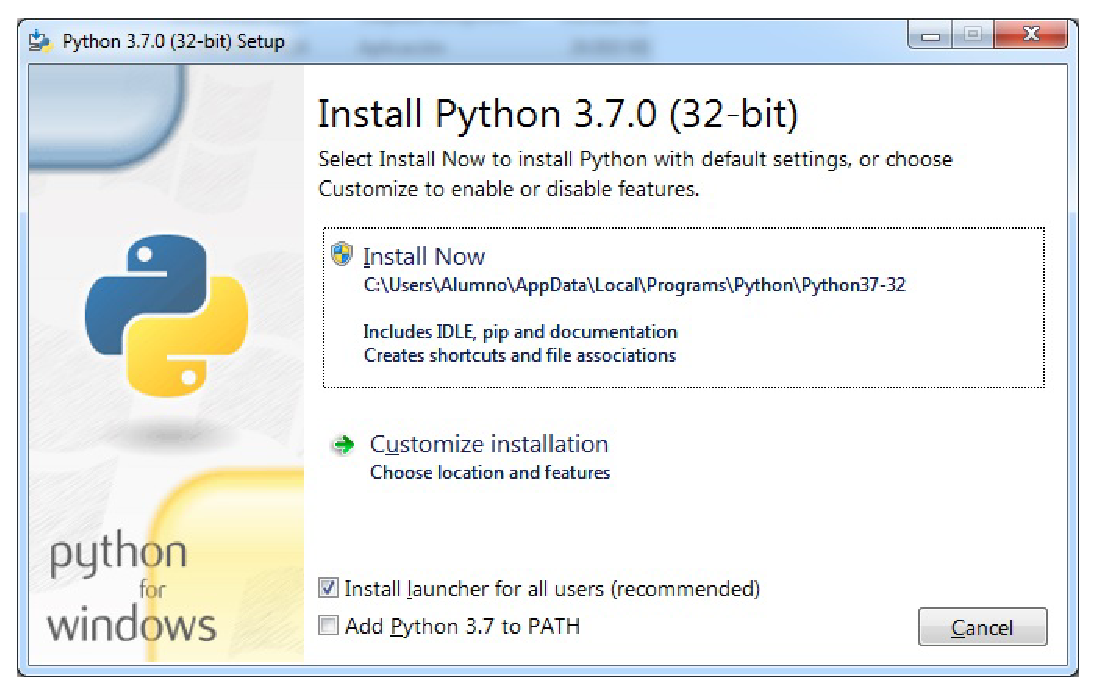
\includegraphics[height=0.5\textwidth]{imagenes/windows}
\end{center}
\caption{Instalación en Windows}
\label{fig:windows}
\end{figure}

\subsubsection{Mac OS X}

Ten en cuenta que un sistema Mac OS X ya tiene alguna versión de Python instalada. Lo más normal es que sea alguna versión de Python 2, como la 2.6 o la 2.7. No pasa nada por tener dos versiones distintas de Python. En la sección \ref{sec:eclipsePython} veremos cómo hay que indicarle al entorno de desarrollo cuál es la que nos interesa usar.

Para este sistema, tenemos dos opciones de instalación de Python 3.7.0 (ver figura \ref{fig:instalacion}): el instalador para Mac OS X 10.9 y versiones posteriores (\emph{macOS 64bit installer}), o el instalador de versiones anteriores del sistema operativo (\emph{macOS 64bit/32bit installer}). Después de la instalación, en el listado de aplicaciones del sistema podremos encontrar una carpeta Python 3.7 que tendrá accesos a:
\begin{itemize}
	\item Integrated Development and Learning Environment (IDLE).
	\item Python Documentation (tutorial del lenguaje, manual de módulos y paquetes, e instrucciones sobre la gestión de los mismos).
	\item Python Launcher. Permite configurar el intérprete que ejecuta los scripts de Python al abrirlos desde Finder.
\end{itemize}

\subsubsection{Linux}

Para instalar Python en Linux, lo más conveniente es usar el comando que gestiona la instalación de paquetes desde un terminal. Por ejemplo, en Ubuntu se haría así:

\begin{lstlisting}
sudo apt-get update
sudo apt-get install python3
sudo apt-get install python3-pip
\end{lstlisting}

Es posible que el comando anterior nos indique que ya tenemos instalada la versión más reciente de Python. Quizás no es la 3.7.0, sino la 3.5.2 o similar. Será suficiente para el desarrollo de las prácticas de la asignatura. La última instrucción instala la herramienta de gestión de paquetes de Python. En caso de usar Fedora, la instalación es muy similar salvo que se debe usar \texttt{yum} en lugar de \texttt{apt-get}.

Con lo anterior, podremos ejecutar desde un terminal el comando \texttt{python3} y se iniciará el intérprete de Python.

\subsection{Eclipse y Python}\label{sec:eclipsePython}

En Autómatas y Lenguajes Formales, vamos a usar Eclipse como entorno de programación de Python. Habitualmente se emplea en la asignatura Programación Orientada a Objetos para el lenguaje Java, de modo que podemos reforzar el manejo de esta herramienta en dos asignaturas. 

Empezamos con la descarga de Eclipse Photon (última versión en el momento de escribir este manual), desde \url{http://www.eclipse.org/photon/}. Al lanzar el instalador de Eclipse, podemos indicar el tipo de entorno que queremos instalar. Las opciones son múltiples, pero ninguna de ellas indica nada sobre Python. Que no cunda el pánico. Se puede instalar una versión para Java (o para C/C++) y luego se modifica para la programación con Python. Recomendamos la primera opción, porque serviría para tener una instalación de Eclipse para las dos asignaturas que emplean este entorno de programación.

Si iniciamos Eclipse después de la instalación, una vez que se indica la ruta al espacio de trabajo (workspace)\footnote{Sería recomendable tener dos espacios de trabajo, uno para Java y otro para Python}, podemos pasar a instalar el plugin que permite emplear Eclipse con Python. Se denomina PyDev, y no hace falta descargarlo e instalarlo independientemente; se puede hacer desde Eclipse, siguiendo estos pasos:

\begin{enumerate}
	\item Entra en el menú \emph{Help}, opción \emph{Install New Software...}
	\item En el campo \emph{Work with:} escribe \texttt{http://www.pydev.org/updates} y pulsa \emph{Enter}.
	\item Marca el paquete \emph{PyDev} y seguidamente pulsa el botón \emph{Next >} dos veces.
	\item Acepta los términos de la licencia del plug-in (Eclipse Public License) y completa la instalación pulsando en \emph{Finish}.
	\item Pulsa en \emph{Restart Now} para que los cambios de Eclipse tengan efecto.
\end{enumerate}

Todavía quedan cosas por hacer. Tenemos que crear un primer proyecto para indicar al plugin PyDev cuál es el intérprete de Python que tiene que usar. Afortunadamente, esto hay que hacerlo sólo al crear el primer proyecto. Seguimos estos pasos:

\begin{enumerate}
	\item En Eclipse, entra en el menú \emph{New} opción \emph{Project}.
	\item Selecciona en el cuadro de diálogo, en la carpeta \emph{PyDev}, el ítem \emph{PyDev Project}. 
	\item Escribe cualquier nombre para el proyecto, como \emph{helloWorld}.
	\item Comprueba que en \emph{Project type} está marcado \emph{Python}. 
	\item En el mismo cuadro de diálogo de creación del proyecto, tendrás que configurar el intérprete de Python que has instalado siguiendo los pasos de la sección anterior. Eso se realiza pulsando donde indica \emph{Please configure an interpreter before proceeding}. 
	\item Selecciona \emph{Advanced Auto-Config} y deja que Eclipse busque las distintas versiones instaladas en el sistema y te permita seleccionar la que quieras usar. Selecciona la versión mayor (\emph{python3.7} o \emph{python3.5} según el sistema). 
	\item A continuación, Eclipse te indicará qué carpetas será necesario añadir al \emph{path} de Python para encontrar los paquetes (librerías) que vas a usar en el código fuente. Pulsa \emph{Ok} al listado por defecto que nos ofrece Eclipse. 
	\item Volviendo al cuadro de diálogo de creación del proyecto, comprueba que en \emph{Grammar Version} aparece seleccionada la opción \emph{Same as interpreter}. 
	\item Pulsa \emph{Finish} para terminar de crear el proyecto. 
\end{enumerate}

Al terminar, veremos que Eclipse muestra dos \emph{perspectivas} para ver el código en iconos arriba a la derecha del entorno de desarrollo: Java y Python. Deberá estar seleccionada esta segunda mientras editemos código Python. La creación de los siguientes proyectos de Python no va a necesitar repetir los pasos para configurar el intérprete de Python, puesto que Eclipse reutilizará esta configuración. Simplemente, bastará con introducir el nombre del proyecto.

\subsubsection{Un paso más en Windows}

Si estás usando Mac OS X o Linux, enhorabuena, ya has terminado con la instalación. Pero si estás con Windows, falta un pequeño detalle que tiene que ver con la codificación usada en ese sistema operativo para los caracteres. Windows emplea un código de caracteres propio, llamado \emph{cp1252}, que no termina de convencer al compilador de Python. Para no tener problemas con los caracteres acentuados, ñ, etc, será mejor que configures el espacio de trabajo de Eclipse para usar \texttt{utf-8} como código de caracteres. Atención: recuerda que te hemos recomendado que crees un espacio de trabajo para Python distinto del que puedas tener para Java. Este cambio podría afectar a tus proyectos Java si estuviesen en el mismo espacio de trabajo que el de Python.

Entra en el menú \emph{Window -> Preferences -> General -> Workspace} y busca al final del cuadro de diálogo \emph{Text file encoding}. Selecciona en \emph{Other} la opción \emph{UTF-8}. Es importante que no edites los ficheros de tus proyectos en Windows con un editor distinto a Eclipse, porque podría estar usando la codificación por defecto de Windows, e intentaría abrir tus ficheros con ella. El lío que se puede montar con los caracteres no ingleses puede ser bastante desagradable.

\clearpage{\pagestyle{empty}\cleardoublepage}

% Capítulo 2: Fundamentos
%!TEX root = Python.tex

\chapter{Fundamentos de Python}

\lettrine[lines=5]{C}{on} el entorno de desarrollo ya configurado, y partiendo del proyecto \emph{helloWorld} creado al final del capítulo anterior, podemos empezar a estudiar el funcionamiento del lenguaje. No es nada original el comienzo que proponemos, porque consiste en el típico programa que imprime \emph{¡Hola mundo!} Algunos manuales de Python introducen innumerables características del lenguaje basándose en el uso interactivo del intérprete, antes de dar la pauta sobre cómo escribir un programa ejecutable. No parece buena idea para estudiantes de Informática que necesitarán escribir aplicaciones desde el comienzo. Así que seguiremos el enfoque clásico.

Pero antes de comenzar, es necesaria una pequeña aclaración sobre la terminología de Python: llamaremos \emph{módulo} a un fichero fuente Python con extensión \texttt{.py}. Este módulo también tendrá un fichero asociado con extensión \texttt{.pyc} una vez que haya sido compilado. Cuando un programa empiece a tener cierto tamaño, será conveniente dividir su código en varios módulos, pero veremos que existe una forma sencilla de reutilizar las funciones de unos módulos en otros. Por otra parte, llamaremos \emph{paquete} a un conjunto de módulos con alguna funcionalidad común. Un paquete es lo mismo que una librería en otros lenguajes de programación y, de hecho, emplearemos indistintamente ambos términos.

\section{Un programa básico}\label{sec:programa_basico}

Un programa básico de Python necesita, al menos, un módulo. Esto es de una lógica aplastante. Los pasos que necesitamos dar desde Eclipse para crear un nuevo módulo son los siguientes:

\begin{enumerate}
	\item Selecciona el proyecto en el que quieres crear el nuevo módulo. Supongamos que es \emph{helloWorld}.
	\item En el menú \emph{File}, usa la opción \emph{New} y la subopción \emph{PyDev Module}.
	\item Deja vacío el campo \emph{package}, que nos serviría para crear un módulo dentro de un paquete (todo a su tiempo).
	\item Indica el nombre del módulo, que puede ser \emph{hello}.
	\item Eclipse nos ofrece varias plantillas (templates) que pueden servir como base para la creación del nuevo módulo. Escoge \emph{Module: Main}.
\end{enumerate}

Después de lo anterior, Eclipse nos muestra un fichero con el siguiente contenido:

\begin{lstlisting}
'''
Created on 5 ago. 2018

@author: jmjuarez
'''

if __name__ == '__main__':
    pass
\end{lstlisting}

\subsection{Comentarios en Python}\label{sec:comentarios}

Hay unas cuantas cosas raras en el fichero. Para empezar, que un tal \emph{jmjuarez} esté el 5 de agosto escribiendo un manual de Python. Pero vayamos a lo importante. En primer lugar, entre las líneas 1 y 5 aparece un comentario limitado por las dos marcas \texttt{'{}'{}'{}}. Es un comentario que puede ocupar varias líneas y sirve para documentar el código. Alternativamente se podría haber usado como limitador del comentario \texttt{"{}"{}"{}}. Trataremos la documentación de código Python más adelante. 

Otra forma de poner comentarios en un programa Python es usando la marca \texttt{\#}. Permite generar comentarios de una línea, o más concretamente, desde la marca hasta el final de la línea.

\subsection{Punto de entrada de un módulo}

Lo siguiente que debe resultar extraño es la línea 7 del código anterior. Para ir aclarando cosas, este código no tiene ninguna función. En Python puedes escribir código fuera de funciones. Esta es una característica de muchos lenguajes interpretados. Esto significa que, al ejecutar el módulo anterior, se alcanza directamente la línea 7, que contiene un \texttt{if}. Vamos posponiendo cosas sin parar, pero una vez más, queda para un apartado posterior la explicación de las sentencias de control de flujo. 

Hay que volver a la idea de módulo para explicar bien la funcionalidad de esa línea. En Python, cualquier módulo puede ser un punto de entrada al programa, es decir, cualquier módulo puede tener el código \emph{principal} del programa. Esto no sucede con C o C++. De hecho, si pusiésemos la función \emph{main()} en todos los ficheros de un proyecto en C, el compilador se quejaría diciendo que la función está repetida por todos sitios.

La explicación de por qué en Python podemos tener múltiples puntos de entrada es sencilla: el lenguaje se pensó para desarrollar \emph{scripts}, es decir, pequeños programas autocontenidos en un módulo. Pero tranquilo, que se puede reutilizar el código de un módulo en otro. Una ventaja de esta característica del lenguaje es que facilita el desarrollo de aplicaciones basado en pruebas. En cada módulo, puedo añadir un código de prueba de las funciones de ese módulo, y podré verificar si todo va bien seleccionando el módulo y ejecutándolo en Eclipse. Cuando haya hecho todas las verificaciones oportunas, podré pasar a usar el módulo importando sus funciones en otro módulo, y así sucesivamente. Siempre habrá, claro está, un módulo final con el programa principal general que servirá para lanzar toda la aplicación.

Y por fin, la explicación de la misteriosa línea 7: este doble uso de los módulos de Python se puede distinguir en tiempo de ejecución, usando la variable predefinida \texttt{\_\_name\_\_}. Esta variable toma el valor \texttt{\_\_main\_\_} cuando un módulo se ejecuta como punto de entrada principal. En Eclipse lo puedes hacer seleccionando el módulo y pulsando en el botón de ejecución; cuando un módulo se importa desde otro módulo para hacer llamadas a sus funciones, esta línea 7 también se ejecuta, pero la variable \texttt{\_\_name\_\_} toma como valor el nombre del módulo importado, de forma que no se ejecuta nada en este caso.

En la línea 8, PyDev introduce la sentencia \texttt{pass}. ¡Esta sentencia no hace nada! Se puede colocar en una parte del código que, en algún momento, tendrá que ser completada. Por ahora, la sustituimos por una sentencia para imprimir \texttt{¡Hola Mundo!} con una llamada a la función \texttt{print}:

\begin{lstlisting}
'''
Created on 5 ago. 2018

@author: jmjuarez
'''

if __name__ == '__main__':
    print('¡Hola Mundo!')
\end{lstlisting}

\subsection{Indentación}

Queda una cosa más, de las raras, pendiente de comentar, que en un programa tan pequeño como \texttt{hello.py} no llama la atención, pero en uno grande sí lo haría: el hecho de tener que poner la llamada a la función \texttt{print} donde está, después de un \emph{tabulador}\footnote{En realidad, el tabulador se convierte en 4 espacios en blanco en un editor como Eclipse.} al comienzo de la línea 8. 

Python no usa palabras clave como \texttt{begin} y \texttt{end} de Pascal, o signos como \texttt{\{} y \texttt{\}} de C y Java, para delimitar bloques de sentencias. ¡Python te obliga a que los delimites con tabuladores! No es válido un programa Python que no respete esa forma de escritura. Esto tiene una ventaja: el código resulta mucho más legible, y eso es algo que puede simplificar mucho la vida de los profesores que tienen que revisar las prácticas.

Por cierto, la palabra \emph{indentación} que introduce esta sección no existe en español, la RAE te lo puede certificar. En su lugar se usa \emph{sangrado}, pero dada la extensión del uso de \emph{indentación}, y teniendo en cuenta que no queremos hacer un manual de Python excesivamente cruento\footnote{Ahora se entiende bien aquello de que \emph{la letra con sangre entra}, que en estos apuntes podríamos reescribir como \emph{Python con sangre entra}.}, nos permitimos la licencia de desobedecer a los reales académicos.

En fin, nadie dijo que los comienzos fuesen fáciles. Pero ahora podemos seguir un camino algo más sistemático para hablar del lenguaje. El resto del capítulo lo dedicamos a esas cosas que tanto nos gusta estudiar cuando aprendemos un lenguaje nuevo: tipos de dato básicos, uso de variables, operadores y sus precedencias, estructuras de control, etcétera. Puedes ir probando todos los ejemplos de los siguientes apartados en el módulo \texttt{hello.py}, pero ¡acuérdate de los tabuladores!

\section{Tipos básicos}\label{sec:tiposBasicos}

\subsection{Enteros}

Existen dos tipos de enteros en Python: \texttt{int} y \texttt{long}. Los primeros tienen una precisión de 32 bits (si el sistema es de 32 bits) o 64 bits (si es de 64). Los segundos, tienen precisión ilimitada, es decir, el único límite es la memoria de tu equipo. Por ejemplo, no hay problema en escribir:

\begin{lstlisting}
print(987987987987987987987987987987987987987+1)
\end{lstlisting}

Así que ya puedes programar esos cálculos astronómicos para los que no habías encontrado un lenguaje adecuado. No será necesario indicar si tu entero es \texttt{int} o \texttt{long}. Dependiendo de su tamaño, Python lo tratará de una forma u otra de manera implícita.

Puedes especificar un signo al comienzo del entero, ¡incluido el positivo! También puedes usar una notación distinta de la base 10, añadiendo delante del entero el prefijo que denota la base, como \texttt{0b} para notación binaria, \texttt{0o} para octal y \texttt{0x} para hexadecimal. Las letras b, o y x pueden estar en mayúsculas.

\begin{lstlisting}
print(0b101)
print(0o101)
print(0x101)
\end{lstlisting}

\subsection{Reales}

Puedes usar valores reales (flotantes) usando la notación clásica (parte entera, separador \texttt{.} y parte decimal), o bien la notación científica con el exponente indicado tras el caracter \texttt{e}:

\begin{lstlisting}
print(-3.1416)
print(44.10e+3)
print(7.5e-4)
\end{lstlisting}

La notación científica es la misma que usa Java, y está definida en el estándar \emph{IEEE 754}.

\subsection{Complejos}

Python es un lenguaje muy apreciado por los programadores que hacen cálculo científico. Y es perfectamente comprensible, porque además de poder hacer cálculos con enteros largos y reales con alta precisión, el lenguaje incluye como tipo básico a los números complejos, usando la notación \emph{<parte real>+<parte imaginaria>j}. En Python ganaron los físicos a los matemáticos en la notación de los complejos. Por ejemplo:

\begin{lstlisting}
print((1+3j)+(2+5j))
\end{lstlisting}

Podemos recuperar la parte real y la parte imaginaria del número complejo:

\begin{lstlisting}
z = 1+3j
print(z.real)  # 1
print(z.imag)  # 3
\end{lstlisting}

\subsection{Cadenas de caracteres}

Python tiene múltiples formas de representar las cadenas de caracteres. Habrás observado que, en el ejemplo de \texttt{hello.py}, la cadena usada es \texttt{'¡Hola Mundo!'}. Igualmente se podría haber empleado \texttt{"¡Hola Mundo!"}. Lo importante es que, si empiezas la cadena con una comilla simple, debes terminarla con una comilla simple, y de forma similar con las comillas dobles.

En realidad, hay una diferencia curiosa entre usar una comilla simple o doble para delimitar una cadena: si quieres que tu cadena incluya caracteres de comillas simples en su contenido, no hay problema, usas comillas dobles al comienzo y final, y viceversa:

\begin{lstlisting}
print("Esto es 'curioso', ¿no?")
print('Vaya "rarezas" tiene Python')
\end{lstlisting}

Siempre es posible usar caracteres de escape dentro de las cadenas de caracteres, antecedidos con la contrabarra, como:

\begin{lstlisting}
print("Esto es una cadena al \"estilo\" de C\n")
print("---\t---")
\end{lstlisting}

Observa que la función \texttt{print}, tal y como la usamos por ahora, introduce un salto de línea al final de la cadena aunque no lo indiquemos con \texttt{$\backslash$n}. También es posible hacer que una cadena ocupe varias líneas usando tres comillas simples (o dobles) en los extremos:

\lstset{language=C}

\begin{lstlisting}
print('''Ahora empezamos por aquí y
continuamos hasta aquí''')
\end{lstlisting}

\lstset{language=Python}

Sí, eso mismo es lo que se usa en los comentarios multilínea para documentar el código, pero aquí el intérprete de Python comprenderá que estamos especificando la cadena que debe imprimir.

Para terminar este apartado, hay una notación adicional para representar cadenas de caracteres que va a ser interesante al definir expresiones regulares\footnote{Gran parte del trabajo de prácticas consistirá en el uso de una representación de patrones de cadenas de caracteres, expresados con una notación formal que se denomina \emph{expresión regular}.}: las cadenas \emph{raw}. Podríamos traducirlo como cadenas \emph{en bruto} o \emph{crudas}. Una cadena de este tipo tiene que ir precedida de \emph{r} o \emph{R}, y especifica que los caracteres de escape no se procesan, es decir, que el carácter de contrabarra $\backslash$ se deja intacto en la cadena. Por ejemplo:

\begin{lstlisting}
print(r'\d\t\d')
\end{lstlisting}


\subsection{Boolean}

Python ofrece un tipo básico \emph{boolean}\footnote{Otra vez nos saltamos la RAE. En el ámbito informático, estamos acostumbrados.} para representar los valores de verdad: \texttt{True} y \texttt{False}. Hay otros valores, como los enteros 1 y 0, que Python permite que se usen con el mismo sentido que \texttt{True} y \texttt{False}. 

\subsection{None}

Y para completar los tipos básicos, Python incluye la posibilidad de representar la \emph{ausencia de valor}. Puede ser útil cuando, en una función, no se devuelve nada porque no se cumplen las condiciones para hacer la operación que se requiera. El modo de representar esa ausencia de valor es \texttt{None}. Las comparaciones son odiosas, y entre lenguajes de programación más todavía, porque dan lugar a discusiones apasionadas pero, salvando las distancias, \texttt{None} vendría a ser algo parecido al \texttt{NULL} de C.

\subsection{Conversiones de tipos}

Muy frecuentemente nos encontraremos con la necesidad de convertir una cadena de caracteres a otro tipo de dato con el cual podamos hacer operaciones aritméticas. Python nos permite hacerlo con una serie de funciones integradas en el propio lenguaje (no hay que importar ninguna librería):

\begin{lstlisting}
x = int("123") # Convierte una cadena en entero corto
y = float("1.2e-3") # Convierte una cadena en real
z = complex("1+2j") # Convierte una cadena en complejo
\end{lstlisting}

Siempre podemos verificar el tipo de cualquier variable o valor con la función \texttt{type()}:

\begin{lstlisting}
z = 1+2j
print(type(z)) # Indica <class 'complex'>
\end{lstlisting}

Las funciones de conversión de tipos que acabamos de ver (usando \texttt{int()} y similares) pueden emplearse pasando como argumento otros valores que no sean cadenas de caracteres. Hay que llevar cuidado con la posible pérdida de información. Por ejemplo:

\begin{lstlisting}
y = 1.2e-3
x = int(y)
print(x)   #  Imprimirá 0
\end{lstlisting}

Los anteriores son ejemplos de conversiones \emph{explícitas}. Sin que haga falta indicar nada, Python puede realizar conversiones \emph{implícitas} de tipos. Por ejemplo:

\begin{lstlisting}
x = 1.2e-3
y = 3
z = x + y  # Se convierte el entero de y en un real antes de sumar
\end{lstlisting}

\subsection{Comprobaciones de tipos}\label{sec:comp_tipos}

Al no tener declaración de variables con tipos, es posible que a una parte de nuestro código Python llege un valor que no tengamos ni idea del tipo que tiene. Si nuestro código tuviese que hacer algo en función del tipo del valor, necesitaríamos una forma de comprobar cuál es. Afortunadamente Python nos ofrece la función integrada en el lenguaje \texttt{isinstance()}. Tiene dos argumentos: un valor y un tipo; y devuelve \texttt{True} o \texttt{False}:

\begin{lstlisting}
print(isinstance(34,int))
\end{lstlisting}

Con los tipos que hemos visto hasta ahora, el segundo argumento -- que coincidiría con lo devuelto por la función \texttt{type()} -- puede ser alguno de los siguientes:

\begin{tabular}{c|l}
	Tipo & Descripción\\
	\hline\hline
	\texttt{int} & Entero\\
	\texttt{float} & Reales\\
	\texttt{complex} & Complejos\\
	\texttt{str} & Cadenas de caracteres\\
	\texttt{bool} & Valores lógicos\\
	\hline
\end{tabular}

\section{Variables}

En Python, las variables no tienen que ser declaradas antes de su uso, como sucede en muchos otros lenguajes de programación como Pascal, Java y C. Algunos opinan que esto puede dar lugar a errores en la programación difíciles de detectar. Todo depende del cuidado que se lleve al programar.

Las variables pueden tener nombres arbitrariamente largos (lo que la memoria de tu equipo y tu capacidad de comprensión te dejen). Pueden contener letras, números y el carácter \texttt{\_}, con la restricción de que comiencen con letra o \texttt{\_}. Las letras pueden ser mayúsculas y minúsculas, y Python distingue un uso u otro. Además, Python 3 permite que uses cualquier letra Unicode en los nombres de las variables, incluyendo vocales acentuadas y ñ. ¡Se acabaron las excusas por las faltas de ortografía al usar términos del español como variables!\footnote{No habría que abusar de los caracteres españoles si vas a compartir tu código a nivel mundial.}

Python, como otros lenguajes, tiene \emph{palabras reservadas} para especificar estructuras de control, operadores, funciones básicas y algunas constantes. En la versión 3 de Python se definen las siguientes 33 palabras reservadas, ordenadas alfabéticamente, siempre en minúscula, salvo tres que contienen una mayúscula:

\begin{multicols}{5}
\begin{verbatim}
and
as
assert
break
class
continue
def
del
elif
else
except
False
finally
for
from
global
if
import
in
is
lambda
None
nonlocal
not
or
pass
print
raise
return
True
try
while
with
yield
\end{verbatim}
\end{multicols}

Para empezar a usar una variable, basta con darle un valor. De hecho, la asignación de un valor a una variable por primera vez corresponde a su \emph{definición}. Si no se hace esto primero, Python nos va a indicar que es erróneo el uso de la variable. La asignación en Python se indica con \texttt{=} entre la variable y el valor:

\begin{lstlisting}
n = 10
print(n)
\end{lstlisting}

Python permite asignaciones múltiples de dos formas. Para dar el mismo valor a varias variables, podemos encadenar las asignaciones:

\begin{lstlisting}
a = b = c = 10
\end{lstlisting}

Otra posibilidad es dar distinto valor a las variables. En este caso, se separan con comas a ambos lados de la asignación las variables y los valores:
\begin{lstlisting}
a, b, c = 2, 4, 16
\end{lstlisting}

Los lenguajes que obligan a declarar las variables antes de su uso, imponen que las variables deban tener el mismo tipo de dato siempre\footnote{Dejamos al margen el tipado dinámico que se logra con la herencia en los lenguajes orientados a objetos.}. Estos lenguajes se denominan \emph{estáticamente tipados}. Python, por el contrario, no tiene esta restricción:

\begin{lstlisting}
a = 23.5
print(a)
a = "Y ahora soy una 'cadena de caracteres'"
print(a)
\end{lstlisting}


\section{Operadores}

Una vez que hemos visto los valores literales y las variables, realizamos ahora un recorrido por los operadores principales del lenguaje que permiten la manipulación de esos elementos en expresiones, agrupándolos en tres bloques: operadores aritméticos, operadores relacionales (comparaciones) y operadores lógicos\footnote{Como \emph{quien mucho abarca poco aprieta}, tenemos que dejarnos muchas cosas en el tintero. Por ejemplo, los operadores a nivel de bit.}.

\subsection{Operadores aritméticos}

La siguiente tabla muestra un resumen de los operadores aritméticos de Python, ordenados de menor a mayor precedencia. Cada sección horizontal representa la misma precedencia. Por ejemplo, la suma y la resta tienen igual precedencia.

\begin{tabular}{c|l}
	Operador aritmético & Descripción\\
	\hline\hline
	$x+y$ & suma\\
	$x-y$ & resta\\
	\hline
	$x*y$ & multiplicación\\
	$x\,/\,y$ & división\\
	$x\,//\,y$ & división entera\\
	$x\%\,y$ & módulo\\
	\hline
	$+x$ & más unario\\
	$-x$ & menos unario\\
	\hline
	$x*\!*\, y$ & potencia
\end{tabular}

Atención: el resultado de la división de enteros es siempre un número real, ¡incluso si el dividendo es divisible por el divisor! En cuanto a la división entera, si el resultado es positivo, se trunca la porción decimal, dejando sólo la entera. Pero si el resultado es negativo, el resultado se redondea al siguiente entero menor:

\begin{lstlisting}
print(10/2)   # El resultado es 5.0
print(10/4)   # El resultado es 2.5
print(10//4)  # El resultado es 2
print(-10//4) # El resultado es -3
\end{lstlisting}

La precedencia entre los operadores determina el orden en el que Python los ejecuta en caso de encontrar una expresión en la que hay varios. Por ejemplo:

\begin{lstlisting}
print(10+2**3)  # Primero se ejecuta 2**3 y el resultado se suma a 10
\end{lstlisting}

Todos los operadores aritméticos pueden combinarse con la asignación para acortar la notación cuando se usa la misma variable a los dos lados de la asignación:

\begin{lstlisting}
x = 1
x += 1 # Equivalente a x = x + 1
y = 2
y /= 5 # Equivalente a y = y / 5 
\end{lstlisting}

\subsection{Operadores relacionales}\label{sec:relacionales}

Los operadores relacionales, también llamados \emph{operadores de comparación}, nos permiten especificar condiciones booleanas que nos harán falta en sentencias de control de flujo. Todos estos operadores dan como resultado \texttt{True} o \texttt{False}. La siguiente tabla muestra un resumen de estos operadores en Python, que comparten la misma precedencia:

\begin{tabular}{c|l}
	Operador relacional & Descripción\\
	\hline\hline
	$a == b$ & igualdad\\
	$a\, !\!= b$ & desigualdad\\
	$a < b$ & menor que\\
	$a <= b$ & menor o igual que\\
	$a > b$ & mayor que\\
	$a >= b$ & mayor o igual que
\end{tabular}

Atención: las comparaciones de números reales pueden dar lugar a resultados inesperados:

\begin{lstlisting}
x = 1.1 + 2.2
print(x == 3.3) # Imprime False porque x contiene 3.3000000000000003
\end{lstlisting}

Esto tiene que ver con la representación interna en Python de los números reales. En este caso, lo más recomendable es hacer una comprobación de lo próximos que se encuentran los dos números comparados, mediante la función \texttt{abs()}, que devuelve el valor absoluto:

\begin{lstlisting}
tolerancia = 1e-10
x = 1.1 + 2.2
print(abs(x - 3.3) < tolerancia) # Imprime True
\end{lstlisting}

Python permite comparaciones encadenadas, que implícitamente están usando una conjunción, evaluando las comparaciones de izquierda a derecha:

\begin{lstlisting}
a = 1
b = 2
c = 2
print(a < b <= c) # True porque a<b y b<=c
\end{lstlisting}

\subsection{Operadores lógicos}

Llega el turno de tratar los operadores que nos permiten construir condiciones lógicas complejas: conjunción, disyunción y negación. Primero, una pequeña tabla para verlos de un vistazo, incluyendo su precedencia de menor a mayor:

\begin{tabular}{c|l}
	Operador lógico & Descripción\\
	\hline\hline
	x or y & Disyunción\\
	\hline
	x and y & Conjunción\\
	\hline
	not x & Negación
\end{tabular}

La interpretación de los operadores es inmediata cuando los operandos son de tipo booleano. Pero Python permite que usemos operandos que no son booleanos. En general, en el contexto de una expresión booleana, se considera que es falso:
\begin{itemize}
	\item El valor booleano \texttt{False}.
	\item Cualquier valor de un tipo numérico básico que sea cero: 0, 0.0, 0+0j.
	\item Cualquier cadena vacía, como \texttt{'{}'{}}, \texttt{"{}"{}}, y con dos o tres comillas simples o dobles.
	\item El valor \texttt{None}.
\end{itemize}

Cualquier otro valor se considera verdadero en el contexto de una expresión booleana. Usando la jerga de programadores de Python o Javascript, usamos el término \emph{falsy} para referirnos a un valor falso distinto de \texttt{False}, mientras que el término \emph{truthy} lo empleamos para los valores verdaderos distintos de \texttt{True}.

Y visto lo esencial sobre los operadores lógicos, añadimos algunas consideraciones peculiares de Python. En primer lugar, si se usan los operadores \texttt{and} y \texttt{or} con operandos que no son booleanos, el resultado no es \texttt{True} o \texttt{False}, sino:

\begin{tabular}{c||l|l}
	x & x or y & x and y\\
	\hline\hline
	si x es \emph{truthy}  & x & y\\
	\hline
	si x es \emph{falsy} & y & x
\end{tabular}

Aquí tenemos un ejemplo de lo anterior:

\begin{lstlisting}
a = 0
b = 1
c = 2
print(b or c)  # 1
print(a or c)  # 2
print(b and c) # 2
print(a and c) # 0
\end{lstlisting}

¿Qué utilidad podría tener esto? En el caso del operador de disyunción, puede servir para implementar una forma de asignar valores algo distinta a la habitual. Si en una asignación \texttt{y = x} el valor de \texttt{x} es \emph{falsy}, podemos asignar a \texttt{y} un valor por defecto:

\begin{lstlisting}
x = ""
y = x or "valor por defecto"
print(y)
\end{lstlisting}

Esto puede ser interesante para evitar errores en ciertos casos en los que no se puede manejar un valor \emph{falsy}.

Por otro lado, como en la mayoría de lenguajes de programación, las condiciones lógicas complejas que usan conjunciones o disyunciones múltiples se implementan con una evaluación de \emph{cortocircuito}. En el momento en que se verifique que la condición es \emph{True} o \emph{False}, se detiene la evaluación. Esto habrá que tenerlo en cuenta si se usan llamadas a funciones como operandos de la conjunción o disyunción múltiple, ya que la llamada podría no realizarse.

\subsection{Precedencia entre distintos tipos de operador}

¿Qué orden de evaluación emplea Python cuando combino operadores aritméticos, relacionales y lógicos? Al igual que dentro de un mismo tipo de operador existe una precedencia (salvo los relacionales, que tienen todos la misma), entre los distintos tipos también hay un orden de evaluación por defecto: 

\begin{tabular}{l|c}
	Tipo de operadores & Orden de evaluación\\
	\hline\hline
	Operadores lógicos & menor precedencia\\
	\cline{1-1}
	Operadores relacionales & $\downarrow$\\
	\cline{1-1}
	Operadores aritméticos & mayor precedencia
\end{tabular}

En caso de duda, siempre podemos recurrir a los paréntesis para ordenar la evaluación.

\begin{lstlisting}
x = 1
y = False
z = True
print(x+2*4 < 0 or y and -z%1)
# Equivale a (((x+(2*4)) > 0) or (y and ((-z)%1)))
\end{lstlisting}

\section{Estructuras de control}

Y ahora que sabemos lo que Python puede aceptar como expresión lógica, podemos pasar a estudiar la forma de las sentencias que permiten representar estructuras de control: sentencias \texttt{if}, \texttt{while} y \texttt{for}.

\subsection{Sentencia if}

Ya hemos visto en la sección \ref{sec:programa_basico} el uso de un \texttt{if}. Esta estructura de control tiene la forma:

\begin{lstlisting}
if <condición>:
    <sentencias_condición_verdadera>
\end{lstlisting}

donde \texttt{<condición>} es una expresión que se puede interpretar como \emph{falsy} o \emph{truthy}, y las sentencias que se ejecutan cuando se cumple la condición tienen todas ellas un nivel de tabulación adicional al del \texttt{if}. 

Una variante de esta construcción, con un bloque \texttt{else}, tendría esta forma:

\begin{lstlisting}
if <condición>:
    <sentencias_condición_verdadera>
else:
    <sentencias_condición_falsa>
\end{lstlisting}

Si has estudiado la ambigüedad típica de los lenguajes de programación tipo C con las sentencias \texttt{if-else}, comprenderás que en Python no hay ambigüedad posible porque la indentación marca explícitamente cuál es el \texttt{if} con el que está asociado cada \texttt{else}.

Y una tercera variante del \texttt{if} permitiría introducir condiciones alternativas con \texttt{elif}:

\begin{lstlisting}
if <condición1>:
    <sentencias_condición1_verdadera>
elif <condición2>:
    <sentencias_condición1_falsa_y_condición2_verdadera>
	...
else:
    <sentencias_todos_condiciones_falsas>
\end{lstlisting}

Esta tercera variante puede ser útil para implementar algo equivalente a una sentencia \emph{switch-case} de C, porque lo creas o no, ¡en Python no existe! Una de las filosofías del lenguaje es no ofrecer varias formas de hacer lo mismo. 


\subsection{Sentencia while}

Veamos ahora un primer tipo de sentencia de Python para implementar bucles, introducido por la palabra clave \texttt{while}:

\begin{lstlisting}
while <condición>:
    <sentencias_mientras_condicion_verdadera>
\end{lstlisting}

No hay ninguna diferencia notable con respecto al modo de hacer algo similar en C. ¿Y si quiero implementar un \emph{do-while}? Pues nos encontramos con el mismo problema que con las sentencias \emph{switch-case}: no existe en Python. En este caso, la solución podría consistir en usar un esquema como el siguiente (atención, contiene material algo fuerte para puristas de la programación):

\begin{lstlisting}
while True:
    <sentencias_mientras_condicion_verdadera>
    if not <condición>:
        break
\end{lstlisting}

Es decir, la condición del \texttt{while} es siempre cierta, de modo que el bloque de sentencias se ejecuta una vez al menos. La condición de salida \emph{real} del bucle la ponemos al final del bloque de sentencias, con un \texttt{if} que, en caso de cumplirse, ejecuta una sentencia \texttt{break}. La condición de salida es la negación de la condición para continuar en el bucle, obviamente.

La sentencia \texttt{break}, al igual que en C, finaliza el bucle inmediatamente anterior que la contiene. Y para ser completos, indicamos también que Python incluye una sentencia \texttt{continue} para iniciar el siguiente ciclo del bucle que la contiene. Después de esta revisión obligada de aspectos polémicos, exigida por la visión distante que debe acompañar a la enseñanza universitaria, volvemos a un terreno más llevadero.

\subsection{Sentencia for}\label{sec:sentenciaFor}

Ahora sí que vamos a encontrar alguna diferencia con respecto a C. Estrictamente hablando, cualquier \emph{for} de C se puede implementar con un \texttt{while}. Por esta razón, aplicando a rajatabla el criterio de no ofrecer dos formas de hacer lo mismo, las sentencias \texttt{for} de Python son otra cosa distinta. En realidad deberíamos llamarlas sentencias \texttt{for-in}. Esta construcción de Python nos permite hacer un recorrido por los elementos de un conjunto ordenados en una secuencia. 

Supongamos que tengo una lista concreta de valores que quiero manipular por igual. Si la lista es corta, puedo expresarla entre corchetes, separando los valores con comas: \texttt{[$v_1$,$v_2$,$\ldots$,$v_i$]}. La sentencia \texttt{for-in} me permite definir una variable, con el nombre que prefiera, que va a tomar uno a uno el valor de los elementos de esta lista, en la secuencia en que han sido expresados en su definición. Dentro del bloque de sentencias del \texttt{for-in} puedo emplear la variable que actúa como índice:

\begin{lstlisting}
for x in [5,'7',11,'13']:
    print(x,'es un número primo')
\end{lstlisting}

Vemos en el ejemplo que la lista puede contener valores con distinto tipo de dato. También podemos ver que la función \texttt{print} puede llamarse con una lista de argumentos separados por comas que, al mostrarlos por consola, se separan con un espacio en blanco. 

Hay un tipo de dato básico que es una secuencia de valores por sí mismo: una cadena de caracteres. Así que, en Python resulta muy fácil recorrer uno por uno los caracteres de una cadena:

\begin{lstlisting}
a = 0
for c in 'supercalifragilisticoespialidoso':
    print(a,c)
    a += 1
\end{lstlisting}

Una función muy útil para hacer recorridos por secuencias de enteros es \texttt{range()}:
\begin{itemize}
	\item \texttt{range(stop)}: genera una lista de enteros desde 0 hasta \texttt{stop-1}.
	\item \texttt{range(start,stop,step)}: genera una lista desde \texttt{start} hasta \texttt{stop-1} saltando con intervalos dados por \texttt{step}. Si \texttt{step} no se indica, se entiende que el intervalo es 1. Podemos usar un valor negativo en \texttt{step} para generar listas de enteros decrecientes.
\end{itemize}

Un ejemplo de uso de \texttt{range()}:
\begin{lstlisting}
for c in range(0,-10,-1):
    print('c=',c)
\end{lstlisting}

\section{Funciones}

Las funciones de Python se introducen con la palabra clave \texttt{def} seguida del nombre de la función\footnote{Se suele indicar en minúsculas y con guiones bajos separando las palabras: \texttt{destruir\_facultad\_ahora()}.}, los argumentos\footnote{Indistintamente usamos los términos argumento y parámetro.} entre paréntesis separados por comas, y seguidamente dos puntos. Tras la cabecera de la función se inicia su bloque de sentencias, usando la indentación correspondiente. Por ejemplo:

\begin{lstlisting}
def f(a,b,c):
    print('suma=',a+b+c)
\end{lstlisting}

Los argumentos de la función actúan como variables locales del bloque de la función. Igualmente, cualquier variable definida dentro de la función pertenece a un ámbito propio a la función. Por esta razón, se pueden ocultar variables con igual nombre definidas fuera de la función:

\begin{lstlisting}
a = 0

def f():
    a = 5
    print('a',a)

if __name__ == '__main__':
    f()
    print('a',a)
\end{lstlisting}

Sí, estamos de acuerdo, la característica habitual de unos apuntes o un manual sobre un lenguaje es que los ejemplos de código son bastante absurdos. Pero al menos los de estos apuntes sirven para dejar clara la cuestión que se trata en cada momento. En el pequeño trozo anterior tenemos varias cuestiones interesantes. En primer lugar, podemos definir variables \emph{globales} en un módulo, simplemente definiéndolas fuera de una función. En segundo lugar, una función tiene que estar definida antes de ser usada, de forma similar a las variables. Y en tercer lugar, y de esto era de lo que trataba el ejemplo fundamentalmente, la variable global \texttt{a} queda oculta dentro de la función \texttt{f()} por una variable local con el mismo nombre.

Entonces, ¿no hay forma de modificar una variable global desde dentro de una función en Python? La respuesta es que sí, pero requiere que le echemos una mano al compilador de Python para que pueda distinguir este caso. La forma de hacerlo es sencilla: en el bloque de la función hay que introducir una sentencia con la palabra clave \texttt{global} y la lista de variables globales a las que se quiere acceder dentro de la función, separadas por comas:

\begin{lstlisting}
a = 0

def f():
    global a
    a = 5

if __name__ == '__main__':
    f()
    print('a',a)
\end{lstlisting}

El valor devuelto por una función como \texttt{f()} en el ejemplo anterior es \texttt{None}. Para poder devolver un resultado, es necesario emplear la palabra clave \texttt{return}, \emph{nihil sub sole novum}, como dirían los clásicos. Como Python es muy liberal en cuestión de tipos, tienes manga ancha para devolver valores de tipos distintos en la misma función, aunque se recomienda un uso moderado:

\begin{lstlisting}
def f(a):
    if a == 1:
        return 42
    elif a == 2:
        return 1-1j
    elif a == 3:
        return +1e-12
    else:
        return 'And now for something completely different!'

if __name__ == '__main__':
    print(f(1),f(2),f(3),f(4))
\end{lstlisting}


\subsection{Argumentos con valores por defecto}

Una función en cuya definición se indican los parámetros con sus nombres únicamente, requiere que las llamadas tengan exactamente el número de parámetros indicados en la definición. En otro caso, se produciría un error. Pero es muy habitual tener funciones con algún argumento que puede tomar un valor por defecto, de modo que el programador puede evitar pasar siempre ese parámetro a la función. Por ejemplo:

\begin{lstlisting}
def f(a,b,c=0):
    return a+b+c

if __name__ == '__main__':
    print(f(1,2)) # El resultado es 3
    print(f(1,2,3)) # El resultado es 6
\end{lstlisting}

En Python, los argumentos con valores por defecto tienen que estar situados en la parte final de la lista de argumentos. 

\subsection{Invocación con parámetros nombrados}

Python permite que los argumentos de una función no tengan que ser indicados en la llamada en el orden de su definición. Para ello basta con poner en la llamada el nombre del argumento correspondiente seguido de un igual y el valor:

\begin{lstlisting}
def f(a,b,c):
    return a*b+c

if __name__ == '__main__':
    print(f(c=2,a=1,b=3)) # El resultado es 5
    print(f(2,c=0,b=5)) # El resultado es 10
\end{lstlisting}


En el ejemplo anterior vemos que se puede llamar a una función pasando al comienzo argumentos sin nombre seguidos de argumentos con nombre. Los argumentos sin nombre se asignan a los parámetros siguiendo el orden de la definición. Obviamente, no se admiten llamadas que asignen más de un valor a un mismo argumento.

\subsection{No hace falta predeclarar funciones}

Supongamos un código así en C:

\begin{lstlisting}
/* Predeclaro la función a() */
void a();
void b() {
    // Hace algo y entonces llama a a()
    a();
}
void a() {
    // Otra cosa, quizás llamar a b()
}
\end{lstlisting}

El compilador de C necesita la línea 2 con la predeclaración de la función \texttt{a()}, porque en caso contrario fallaría la compilación en la línea 5. Sin embargo, Python no requiere la predeclaración:

\begin{lstlisting}
def b():
    // Hace algo y entonces llama a a()
    a()
}
def a():
    // Otra cosa, quizás llamar a b()
}
\end{lstlisting}

La razón es sencilla: Python no \emph{resuelve} la localización de una función hasta el momento de hacer la invocación. Al llegar a la línea 3, el compilador de Python genera bytecodes que, en el momento de ejecutarse, tendrán que localizar dónde está la función \texttt{a()}, para saltar a su código.


\section{Excepciones}

Cuesta creerlo, pero es necesario aceptar que no somos perfectos. Solemos cometer un montón de errores mientras programamos, que dan lugar a problemas durante la ejecución. Además, la ejecución también puede estar condicionada por los valores que proporciona el usuario, que siempre encontrará la forma de llevar al límite a nuestro programa. Por eso, no viene nada mal que el lenguaje nos ofrezca alguna herramienta para evitar que, cuando hay problemas, todo salte por los aires sin control. En Python esta herramienta son las \emph{excepciones}. 

Vamos a explicarlo con un tipo de error muy básico, pero conforme vayas programando código en Python te darás cuenta de que hay mucha variedad de errores posibles, y para todos ellos hay una forma de representarlos. El caso básico que nos servirá de ejemplo es una división por cero. Supongamos que tenemos un módulo \texttt{c.py} con el siguiente código:

\begin{lstlisting}
def operación(x,y,z):
    return x/y + z

if __name__ == '__main__':
    res = operación(5,0,3)
    print('Resultado =',res)
    print('Finalizando')
\end{lstlisting}

Obviamente no deberíamos escribir un código que va a producir una división por cero tan evidente. Pero imagina que la llamada a \texttt{operación} se realiza con tres variables que proceden de una lectura de teclado. El caso es que, al ejecutar el programa anterior, tendremos un bonito mensaje en la consola:

\begin{lstlisting}
Traceback (most recent call last):
  File "/eclipse-workspace/helloWord/c.py", line 5, in <module>
    res = operación(5,0,3)
  File "/eclipse-workspace/helloWord/c.py", line 2, in operación
    return x/y + z
ZeroDivisionError: division by zero
\end{lstlisting}

Nuestro programa finaliza descontroladamente, pero al menos hay información muy útil en el mensaje de la consola. Empezando por el final, está claro lo que ha pasado: \texttt{ZeroDivisionError: division by zero}. De esa línea nos interesa especialmente el comienzo: \texttt{ZeroDivisionError} es el nombre que Python le da a ese tipo de error, o excepción. Lo usaremos en el código que veremos enseguida para evitar que todo se descontrole. Será importante si estamos implementando el controlador de un reactor nuclear.

Las restantes líneas indican la secuencia de llamadas que ha provocado el problema. En la línea 5 de \texttt{c.py} del código de primer nivel se invoca \texttt{operación} con los argumentos correspondientes; dentro de la función \texttt{operación}, en la línea 2 del mismo módulo, se encuentra la división que lanza la excepción. 

\subsection{Bloque try-except}

Para tener un control sobre los posibles errores en tiempo de ejecución de un programa, y evitar que provoquen la finalización abrupta del mismo, Python nos ofrece una sentencia que funciona, básicamente, con dos palabras clave, \texttt{try} y \texttt{except}, que introducen dos bloques de código. El bloque de \texttt{try} contiene el código en el que, potencialmente, puede producirse la excepción, mientras que el bloque de \texttt{except} incluye el código que \emph{maneja} la excepción. Por ejemplo:

\begin{lstlisting}
if __name__ == '__main__':
    try:
        res = operación(5,0,3)
        print('Resultado =',res)
    except ZeroDivisionError:
        print('Problemas con una división por cero')
    print('Finalizando')
\end{lstlisting}

Detrás de la palabra clave \texttt{except} podríamos haber dejado los dos puntos directamente, sin indicar el nombre de la excepción que queremos capturar. Eso nos permitiría escribir un manejador de errores genérico. Sin embargo, conviene indicar expresamente cuál es la excepción que queremos capturar. En este caso, el tratamiento del error no es ninguna maravilla: un mensaje de error al usuario. Algo más conveniente sería indicarle que reintroduzca los datos para hacer otro intento. Si ejecutas el código anterior, podrás observar que no se llega al \texttt{print} de la línea 4. Es normal: si se produce la excepción en una sentencia del bloque del \texttt{try}, deja de ejecutarse ese bloque y se pasa a ejecutar el bloque del \texttt{except} que especifica la excepción que se ha producido.

\subsection{Bloque try-except-else-finally}

El bloque de tratamiento de excepciones que hemos visto en la sección anterior es un caso de la estructura más completa que podemos usar en Python, y que seguiría la siguiente plantilla:
\begin{lstlisting}
try:
    /* Bloque que puede lanzar excepciones */
except Excepción1:
    /* Tratamiento de las excepciones tipo Excepción1 */
except (Excepción2,Excepción3):
    /* Tratamiento de las excepciones tipo Excepción2 y Excepción3 */
...
except:
    /* Tratamiento de otras excepciones */
else:
    /* Bloque que se ejecuta si no ha habido excepciones */
finally:
	/* Bloque que se ejecuta en cualquier caso al final */
\end{lstlisting}

Como ves, si el tratamiento de varias excepciones va a ser igual, podemos indicarlo listándolas entre paréntesis en un único \texttt{except}. 

\subsection{Aserciones}

Una forma de depurar programas Python es usar la sentencia \texttt{assert}, que permite generar una excepción cuando no se cumple alguna condición necesaria para la correcta ejecución de una porción de código. Por ejemplo:

\begin{lstlisting}
def operación(x,y,z):
    assert y!=0,'Parámetro y es 0'
    return x/y + z

if __name__ == '__main__':
    try:
        res = operación(5,0,3)
        print('Resultado =',res)
    except AssertionError as error:
        print('No se cumple una aserción:', error)
    print('Finalizando')
\end{lstlisting}

La sentencia \texttt{assert} requiere una condición, que se evalúa para comprobar si es \texttt{False}. En este caso, se genera una excepción de tipo \texttt{AssertionError} que contiene el dato que se especifica a continuación de la coma. Esa excepción puede ser capturada y manipulada convenientemente dentro de una estructura \texttt{try-except} del programa. Observa la línea 9 del código anterior. La línea \texttt{except} termina con \texttt{as error}. La palabra clave \texttt{as} permite darle un nombre a la instancia de la excepción \texttt{AssertionError} que se captura en esta línea, y más concretamente el nombre es \texttt{error}. Dentro del bloque que introduce este \texttt{except} se puede usar esta variable para hacer referencia a la excepción. Muy frecuentemente se imprimirá mediante una sentencia \texttt{print()}.



\clearpage{\pagestyle{empty}\cleardoublepage}

% Capítulo 3: Módulos
%!TEX root = Python.tex

\chapter{Módulos y paquetes}\label{chap:modulosPaquetes}

\lettrine[lines=5]{U}{na} de las claves del éxito de Python es la gran facilidad que ofrece el propio lenguaje para la organización del código. Esta organización se construye sobre el concepto de \emph{módulo} que ya hemos introducido, y se extiende con el de \emph{paquete}. La ventaja principal de esta estructura es la reusabilidad de código, que ha dado lugar a la disponibilidad de una gran cantidad de librerías de una comunidad de programadores de Python creciente. En este capítulo analizamos cómo se organiza el código de un proyecto de Python. Aunque las prácticas de la asignatura de Autómatas y Lenguajes Formales no requieran grandes proyectos, no deja de resultar útil conocer el funcionamiento del sistema de módulos y paquetes de Python dadas las ventajas que supone, incluso en proyectos pequeños, gracias a la utilización de librerías.

\section{Dos formas de importar}

Un programa Python consiste en un conjunto de ficheros de código (módulos) de entre los cuales hay uno que contiene el código principal. Para integrar los distintos ficheros entre sí, es necesario usar un mecanismo que permita \emph{importar} las definiciones (funciones o variables) de un módulo en otro módulo. Empezamos considerando el caso más sencillo posible: tenemos dos módulos \texttt{a.py} y \texttt{b.py} que se encuentran en el mismo directorio, y queremos importar definiciones del segundo en el primero. Veamos un ejemplo de un módulo \texttt{b.py} que se va a importar. 

\begin{lstlisting}
# Modulo b.py. Define x y spam
x = 10
def spam(text):
    print(text,'is not')
    i = 0
    while i<x:
        print('spam')
        i += 1
\end{lstlisting}

\subsection{Import}

En Python, podemos realizar la importación de definiciones de un módulo empleando las sentencias del lenguaje \texttt{import} y \texttt{from}. La primera opción, \texttt{import}, permite que \emph{todas} las definiciones de un módulo se incorporen a un segundo módulo, que es precisamente el que contiene la sentencia \texttt{import}. Por ejemplo, el módulo \texttt{a.py} que realiza esta importación puede hacerlo así:\footnote{Como ves, no es necesaria la condición \texttt{if \_\_name\_\_} en el módulo \texttt{b.py}. Estrictamente hablando, tampoco lo es la de \texttt{a.py}, pero conviene acostumbrarse a usarla, ya que podría darse el caso de que \texttt{a.py} pasara a ser importado desde otro fichero \texttt{c.py} que tuviese el código principal.}:

\begin{lstlisting}
# Modulo a.py
import b # Importamos todas las definiciones de b.py

if __name__ == '__main__':
    b.x = 5
    b.spam('zarangollo')
\end{lstlisting}

Observa que las definiciones importadas desde \texttt{b.py} con \texttt{import} se tienen que usar en \texttt{a.py} precediendo el identificador con el prefijo \texttt{b.}, es decir, el nombre del módulo importado sin la extensión \texttt{py}. A esto se le llama \emph{espacio de nombres}, y te resultará familiar de otros lenguajes de programación. Por ejemplo, si en C declaramos una variable cuyo tipo es una estructura, para acceder a los campos de la estructura tenemos que usar el nombre de la variable como espacio de nombres. Con los módulos de Python es similar.

El hecho de que el nombre de un módulo se use como parte del identificador de una definición al usar este tipo de importación, tiene una implicación: los nombres de los ficheros Python deben cumplir las mismas restricciones que los nombres de las variables. 

Si no te gusta el nombre del módulo, por alguna razón, puedes indicar un nombre distinto en el momento de hacer la importación, ampliando la llamada a \texttt{import} con \texttt{as nombre}: 

\begin{lstlisting}
import dijkstra as d # d.x para acceder al identificador x de dijsktra
\end{lstlisting}

\subsection{From - import}

La segunda opción de importación es \texttt{from}. En este caso, podemos especificar qué definiciones queremos importar. Por ejemplo, si quisiéramos usar sólo la función \texttt{spam}\footnote{En los libros y webs sobre Python verás que es frecuente usar ejemplos con \emph{spam}. Tiene su explicación: la palabra adquirió su significado actual por un famoso sketch de los Monty Python que puedes encontrar en Youtube.} de \texttt{b.py}:

\begin{lstlisting}
# Modulo a.py
from b import spam

if __name__ == '__main__':
    spam('zarangollo')
\end{lstlisting}

Si fuesen varias las definiciones importadas, se indicarían separadas por comas. Si se quieren importar todas, se usa un asterisco \texttt{*}. Observa que, en esta segunda forma de importar, ya no es necesario el uso del nombre del módulo \texttt{b} como espacio de nombres de las definiciones importadas. Estas quedan fusionadas en el espacio de nombres por defecto del módulo que recibe la importación. Esto tiene una primera implicación: si importamos desde varios módulos una definición que tiene el mismo nombre, no podremos usar \texttt{from}, sino que tendremos que emplear \texttt{import} para poder distinguir una de otra. Además, al usar \texttt{from}, si tuviésemos una definición con el mismo nombre en el módulo que importa y en el módulo importado, podrían ocultarse una y otra:

\begin{lstlisting}
# Modulo a.py
x = 5
from b import *

if __name__ == '__main__':
    print('x =',x) # Imprime 10 en lugar de 5
\end{lstlisting}


\subsection{Cómo funciona la importación}

Un error frecuente de los programadores de C al llegar a Python es considerar que \texttt{import} y \texttt{from} funcionan de forma similar a \texttt{\#include}. Pero las diferencias son notables: \texttt{\#include} es una directiva de \emph{precompilación}, que sirve para pegar el contenido de un fichero (normalmente un fichero de cabecera {\texttt{.h}) en otro fichero. Sin embargo, \texttt{import} y \texttt{from} son \emph{sentencias} de Python, es decir, operaciones básicas incluidas en el propio lenguaje. Esto supone que pueden aparecer en cualquier sitio en el que sea aceptable una sentencia de Python, y se ejecutan en el momento en que la ejecución llega a ellas.

Además, las dos sentencias de importación de Python realizan tres pasos:
\begin{enumerate}
	\item Encontrar el módulo que se quiere importar.
	\item Compilar a bytecodes el módulo importado, si fuese necesario.
	\item Ejecutar el código del módulo importado.
\end{enumerate}

Vamos a analizar brevemente cada uno de estos tres pasos. 

\subsubsection{Encontrar el módulo}

El ejemplo sencillo de la sección anterior es un caso muy frecuente: el módulo importado está en el mismo directorio que el módulo que realiza la importación. No obstante, podríamos tener una panoplia de situaciones muy variada, en función de la organización del código de nuestro proyecto. Por esta razón, Python define unas reglas de búsqueda para la importación de módulos. El módulo importado se busca sucesivamente en las siguientes localizaciones, por orden:

\begin{enumerate}
	\item Primero se intenta localizar en el mismo directorio del módulo que realiza la importación. Al usar Eclipse, el directorio es el que lleva el nombre del proyecto y se localiza dentro de la carpeta de \texttt{workspace}.
	\item Si lo anterior falla, se consulta el contenido de la variable \texttt{PYTHONPATH}. En el caso de usar Eclipse, esta variable se puede definir accediendo a las propiedades del proyecto (pulsa sobre el nombre del proyecto con el botón derecho del ratón y selecciona \emph{Properties}). La ventana que aparece es similar a la de la figura \ref{fig:pythonpath}. En la pestaña \emph{Source Folders} se pueden indicar otros directorios de proyectos del workspace de Eclipse. En la solapa \emph{External Libraries} podríamos especificar localizaciones en cualquier directorio del sistema, fuera del workspace.
	\item Si todavía no se ha localizado el módulo, se intenta con los directorios que contienen las librerías estándares\footnote{Las librerías estándares son las que están en cualquier instalación de Python, sin necesidad de añadir nada adicional aparte del propio sistema de Python. Permiten hacer muchas operaciones que en otros lenguajes requerirían la instalación de librerías adicionales. Puedes ver un listado completo para Python 3 aquí: \url{https://docs.python.org/3/library/}.} de Python en el sistema.
	\item Por último, Python intenta localizar el módulo en el directorio de librerías adicionales, instaladas con herramientas como \texttt{pip} que luego describimos. El subdirectorio último de esta ruta suele denominarse \emph{site-packages}.
\end{enumerate}

\begin{figure}
\begin{center}
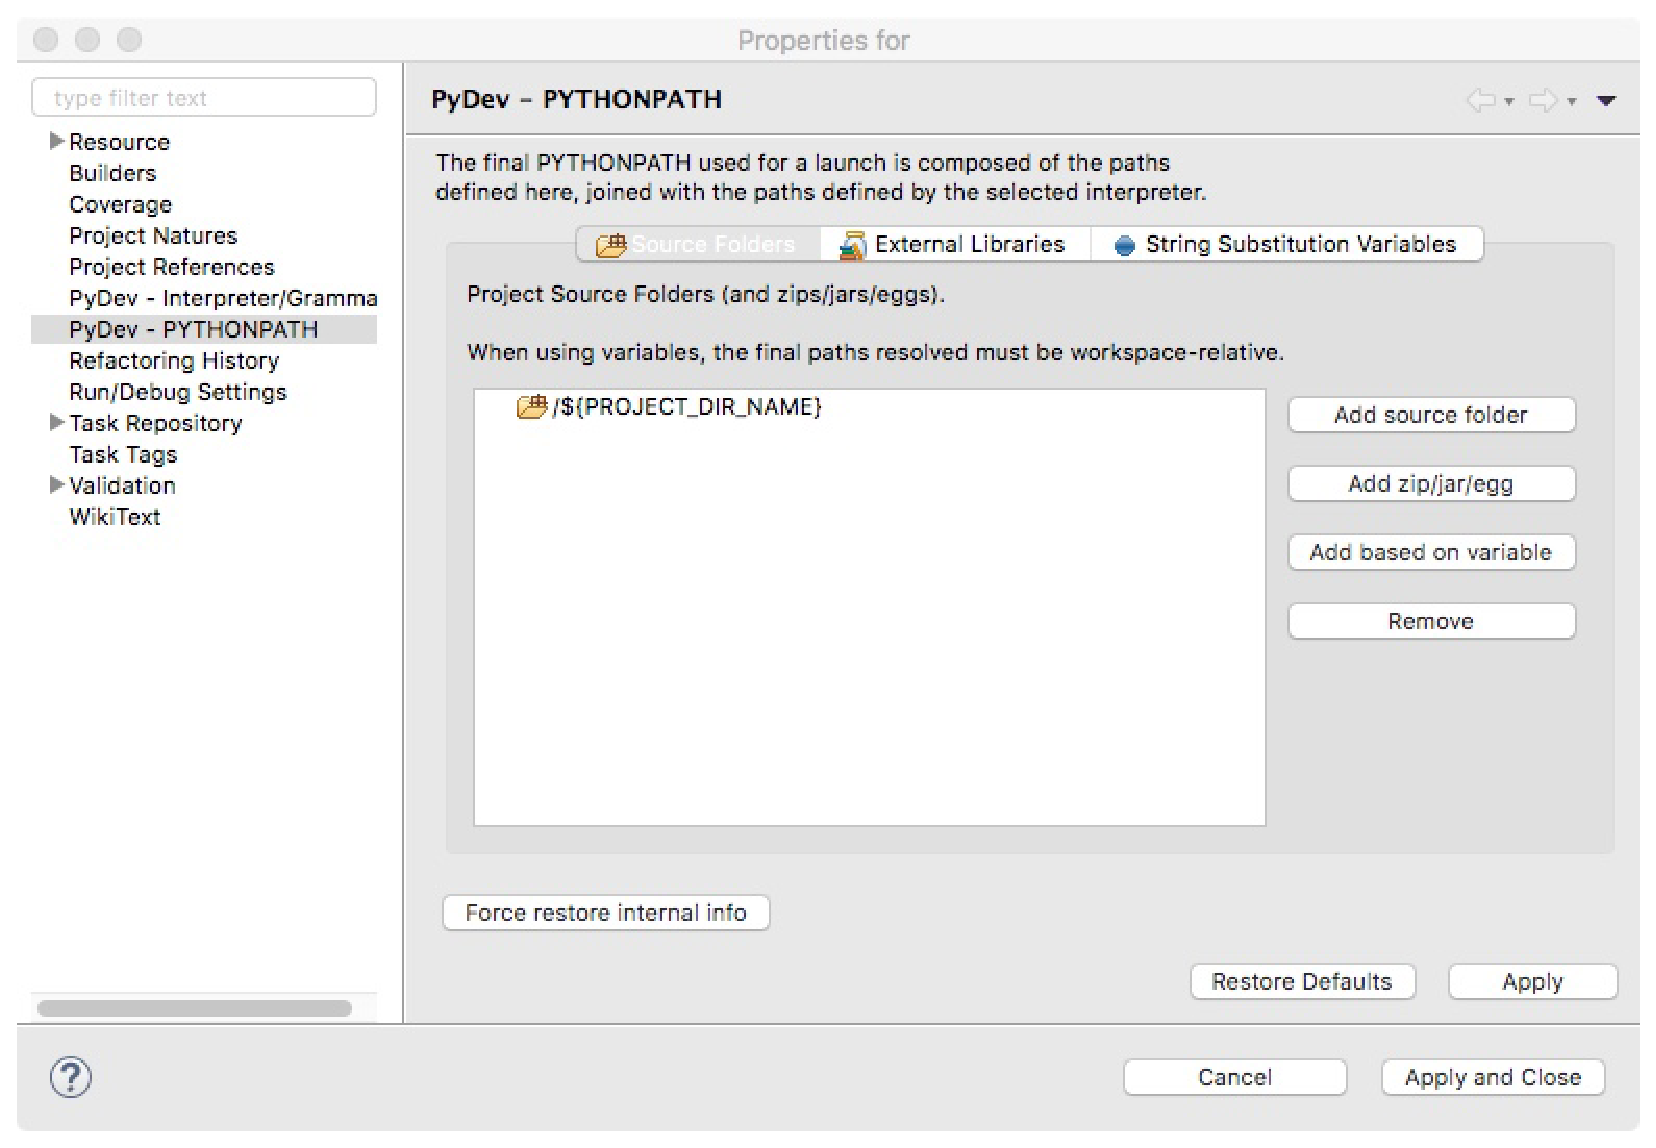
\includegraphics[height=0.45\textwidth]{imagenes/pythonpath}
\end{center}
\caption{Propiedades del proyecto Eclipse para especificar PYTHONPATH}
\label{fig:pythonpath}
\end{figure}

Existe alguna posibilidad adicional después de las anteriores para hacer otro intento de localización, pero no se van a tratar aquí. ¿Y si no se encuentra el módulo? Pues se produce una excepción de tipo \texttt{ImportError}.

\subsubsection{Compilación a bytecodes}

Después de localizar el fichero de código fuente (con extensión \texttt{.py}) del módulo que hay que importar, Python compila el código a bytecodes si es necesario. Para determinar si es necesario, se hace una comparación del instante de última modificación del fichero fuente con el del fichero compilado. Si el primero es posterior al segundo, se realiza la compilación del módulo importado. El resultado es un fichero con extensión \texttt{.pyc} que queda almacenado en el subdirectorio \texttt{\_\_pycache\_\_} dentro del directorio del proyecto.

Ten en cuenta que la compilación sólo se realiza cuando se importa un módulo. Por esta razón, normalmente no verás un fichero \texttt{.pyc} para el módulo principal, a menos que sea importado en otro sitio. ¿Significa esto que el módulo principal no se compila? No, también se compila, pero se hace cada vez que se ejecuta y sus bytecodes no se guardan en ningún sitio, sino que son desechados al finalizar el programa. Conviene que el módulo principal sea lo más pequeño posible para acelerar la ejecución del programa.

\subsubsection{Ejecución del módulo importado}

Hay un último paso en la importación de un módulo: su ejecución. Aquí tienes una buena razón para entender que la importación de módulos de Python no tiene mucho que ver con la directiva de precompilación \texttt{\#include} de C. 

Podemos distinguir dos tipos de código dentro de un módulo: definiciones de funciones y código de \emph{primer nivel}. Las funciones se declaran, como ya hemos visto, con la palabra clave \texttt{def}. En cierta forma podemos considerar que estas declaraciones se \emph{ejecutan} al cargar un módulo en el sentido de que las funciones quedan disponibles para su uso en el módulo que realiza la importación. En cuanto al código de \emph{primer nivel}, se trata de código Python del módulo importado que no forma parte de la definición de funciones. Podríamos considerar que esto de \emph{primer nivel} tiene que ver con el nivel de indentación inicial. Por ejemplo, la inicialización de variables o la típica sentencia \texttt{if \_\_name\_\_ == \_\_main\_\_:} etc., es un caso de código de \emph{primer nivel} de un módulo. Este código se ejecuta al importar el módulo, indistintamente de si se usa \texttt{import} o \texttt{from}.

\subsubsection{Algunas consideraciones más}

Como \texttt{import} y \texttt{from} son sentencias, pueden estar dentro de otras sentencias condicionales. Esto implica que los módulos se puede importar en función de las condiciones que se produzcan durante la ejecución del programa. Por otra parte, es posible realizar varias llamadas de importación de un módulo en el mismo programa. Sólo la primera tendrá como consecuencia la ejecución de los tres pasos que acabamos de ver. Las restantes llamadas de importación reutilizarán el módulo que ya está en memoria.

Cuidado con los nombres de las variables y funciones definidas en un módulo. Si son demasiado generales, como \texttt{x} o \texttt{f}, es posible que tengas montado un buen lío al importar varios módulos en otro si hay coincidencia de nombres y usas \texttt{from}.

\section{Paquetes}

Hasta ahora, sólo hemos visto cómo importar un módulo en otro. Posiblemente, tus primeros desarrollos en Python no necesiten mucho más. Pero, ¿para qué ponerse límites? En el momento en que tus programas Python vayan creciendo, posiblemente necesites una estructura de módulos ordenados en distintos directorios. Aquí es donde viene al rescate el concepto de \emph{paquete} (también lo hemos llamado \emph{librería} en varias ocasiones): un paquete Python no es más que un directorio con una serie de módulos Python, y opcionalmente con subdirectorios (subpaquetes) con más módulos. Sólo hace falta un pequeño detalle para que Python sepa que un directorio es un paquete: debe contener un fichero con el divertido nombre de \texttt{\_\_init\_\_.py}. Ese fichero puede estar vacío, aunque lo normal es que contenga lo siguiente:

\begin{itemize}
\item Código de inicialización del paquete. Por ejemplo, la definición de valores de variables por defecto o la apertura de algún recurso del sistema.
\item Un listado de los módulos que se importan si se usa \texttt{*} en la importación del paquete en una sentencia \texttt{from}. La idea es que quizás no todos los módulos del paquete contienen funciones para ser usadas desde fuera, y sólo queremos que se ejecute la importación de algunos de ellos. El listado se especifica en una variable con el nombre \texttt{\_\_all\_\_}.
\end{itemize}

Supongamos que tenemos un paquete en un directorio llamado \texttt{ordenar}, dentro del cual hay un módulo por cada algoritmo de ordenación: \texttt{bubblesort.py}, \texttt{quicksort.py}, etc. Supongamos que todos estos módulos tienen un método \texttt{sort()} con un argumento que es una lista de enteros, y que el método imprime el resultado de la ordenación.

Dentro del fichero \texttt{\_\_init\_\_.py} del directorio \texttt{ordenar} podemos dar valor a \texttt{\_\_all\_\_} con la lista de módulos que se importan desde el paquete si se usa \texttt{from} con \texttt{*}:
\begin{lstlisting}
# __init__.py del paquete ordenar
__all__ = ["bubblesort","quicksort","mergesort","cocktailsort"]
\end{lstlisting}

A nivel básico, la importación de definiciones de paquetes funciona como con los módulos invididuales, pero ahora usando el nombre del paquete (ruta de directorios) delante:

\begin{lstlisting}
import ordenar.bubblesort
# Uso el método sort del módulo bubblesort
ordenar.bubblesort.sort([5,2,9,34,12])
\end{lstlisting}

El mecanismo de importación realiza la búsqueda del paquete siguiendo el mismo orden de localizaciones posibles que en el caso de los módulos individuales\footnote{Si se importa un paquete contenido dentro de otro paquete, lo importante es localizar al primero, el paquete de más alto nivel, ya que los subpaquetes son subdirectorios del primero.}. Como puedes ver en el código anterior, para invocar al método \texttt{sort} es necesario indicar delante el nombre completo del módulo, incluyendo el nombre del paquete delante. Por esta razón, puede ser conveniente usar \texttt{as} en las sentencias \texttt{import}:

\begin{lstlisting}
import ordenar.bubblesort as bubble
# Uso el método sort del módulo bubblesort renombrado como bubble
bubble.sort([5,2,9,34,12])
\end{lstlisting}

También podemos realizar la importación de un paquete usando la sentencia \texttt{from}:

\begin{lstlisting}
from ordenar import bubblesort
# Uso el método sort del módulo bubblesort
bubblesort.sort([5,2,9,34,12])
\end{lstlisting}

Y si queremos afinar mucho, podemos indicar específicamente el método que queremos usar:

\begin{lstlisting}
from ordenar.bubblesort import sort
# Uso el método sort del módulo bubblesort
sort([5,2,9,34,12])
\end{lstlisting}

Por el contrario, si no tenemos claro qué queremos usar de un paquete, siempre se puede usar una importación a lo salvaje:

\begin{lstlisting}
from ordenar import *
# Uso el método sort del módulo mergesort
mergesort.sort([5,2,9,34,12])
\end{lstlisting}

Observa que, en este último caso, tienes que indicar el módulo delante del método \texttt{sort}	que quieres usar, ya que se han importado todos los módulos indicados en la lista \texttt{\_\_all\_\_} o, en caso de que no esté definida, todos los módulos del paquete.


\subsection{Creación de paquetes en Eclipse}

En la sección \ref{sec:programa_basico} te indicamos cómo se puede crear un módulo dentro de Eclipse. Si le vuelves a echar un vistazo verás que, en el tercer paso, dejamos vacío el campo \texttt{package}. No hace falta ser un genio para darse cuenta de que, si indicamos un nombre de paquete, Eclipse va a crear el módulo dentro de un subdirectorio con el nombre del paquete. Ese subdirectorio se crea en el directorio del proyecto, dentro del \emph{workspace} de Eclipse. Si es el primer módulo de ese paquete, el subdirectorio se crea en ese momento. Si no, simplemente se añade el nuevo módulo.

Existe también la posibilidad de crear un paquete vacío, usando la opción \emph{PyDev Package} dentro del menú \emph{File}, opción \emph{New}.

\subsection{Gestión de paquetes con \texttt{pip}}

Si todo fue correctamente durante la instalación de Python (sección \ref{sec:instalacion}), desde la línea de comandos de tu sistema tendrás la posibilidad de ejecutar el comando \texttt{pip} (podrías necesitar tener permisos de administrador para hacerlo). Es la herramienta básica para acceder al \emph{Python Package Index} (PyPI), el repositorio de paquetes para el lenguaje Python que actualmente cuenta con casi 150000 proyectos\footnote{Puedes acceder a un buscador de paquetes del repositorio en \url{https://pypi.org/}.}.

Lo primero que puede resultar conveniente es actualizar la propia herramienta \texttt{pip} para estar seguros de que tenemos la última versión. Necesitamos usar un comando que es todo un homenaje a la recursión: 

\begin{lstlisting}
pip install --upgrade pip
\end{lstlisting}

Supongamos que, tras buscar un rato en Google, hemos localizado un paquete para reconocimiento de voz que nos interesa usar. El nombre del paquete es \texttt{SpeechRecognition}. Sabiendo el nombre del paquete, la forma de instalarlo es realmente sencilla:

\begin{lstlisting}
pip install SpeechRecognition
\end{lstlisting}

Aparecerá una barra que muestra el progreso de la descarga, y en poco tiempo tendremos instalado el paquete en el equipo. Si eres un poco maniático y quieres tener un control exhaustivo de qué ficheros contiene el paquete que se ha instalado, y exactamente dónde se encuentran, no hay problema, se lo preguntamos a \texttt{pip}:

\begin{lstlisting}
pip show --files SpeechRecognition
\end{lstlisting}

Para saber cuáles son los paquetes que tenemos instalados mediante \texttt{pip}, podemos solicitar un listado de la siguiente forma:

\begin{lstlisting}
pip list
\end{lstlisting}

Junto a cada paquete aparece indicada la versión que tenemos instalada en el sistema. Si quisiéramos ver los paquetes que están desactualizados, podemos hacerlo así:

\begin{lstlisting}
pip list --outdated
\end{lstlisting}

Y si encontramos un paquete desactualizado, podemos actualizarlo a su última versión así:

\begin{lstlisting}
pip install --upgrade paquete
\end{lstlisting}

Desinstalar un paquete es igual de sencillo que instalarlo:

\begin{lstlisting}
pip uninstall paquete
\end{lstlisting}

El comando \texttt{pip} tiene la deferencia de consultarnos si realmente queremos hacer la desinstalación. Si tienes curiosidad, puedes ver que \texttt{pip} se puede hacer el harakiri a sí mismo. 
\clearpage{\pagestyle{empty}\cleardoublepage}

% Capítulo 4: Strings
%!TEX root = Python.tex

\chapter{Cadenas}
\label{chap:cadenas}

\lettrine[lines=5]{L}{as} cadenas (strings) en Python se usan para representar cualquier cosa que pueda ser codificada como texto o bytes. En la parte relativa al texto, las cadenas incluyen símbolos de cualquier alfabeto conocido, empleando para ello el sistema Unicode que permite la representación de todo tipo de caracteres de lenguajes humanos. Y por otro lado, una cadena puede almacenar bytes en crudo para representar contenidos binarios de cualquier tipo, como mensajes de red o ficheros multimedia.

Al comenzar a tratar las cadenas en profundidad, es necesario realizar una aclaración sobre la división que Python realiza entre los tipos de dato que se manejan desde el propio lenguaje: tipos de dato inmutables y mutables.

En Python se denomina \emph{inmutable} a un tipo de dato cuyas instancias no se pueden modificar. Son inmutables los tipos básicos que se describieron en la sección \ref{sec:tiposBasicos}, incluyendo las cadenas. Cualquier operación realizada sobre una instancia de estos tipos no altera la instancia, sino que genera una instancia nueva. En concreto, en el caso de las cadenas, son secuencias de caracteres o bytes con un orden en su posición de izquierda a derecha que no pueden ser modificadas. Por ejemplo, si se quiere concatenar una cadena con otra, se genera una tercera cadena con el resultado de la concatenación, pero no se alteran ninguna de las dos cadenas concatenadas. Sucede de forma similar con todas las operaciones realizables sobre las cadenas, que veremos en este capítulo. En el siguiente capítulo se describen los tipos mutables de listas y diccionarios. 

Además de la creación de cadenas de caracteres que vimos en la sección \ref{sec:tiposBasicos}, es posible crear cadenas binarias anteponiendo el prefijo \texttt{b} a la cadena. Por ejemplo, el siguiente código genera una cadena binaria de dos bytes, el primero con valor 0 y el segundo con valor 255:

\begin{lstlisting}
a = b'\x00\xFF'
\end{lstlisting}

Cada byte se especifica usando el código de escape \texttt{$\backslash$x\emph{hh}}, donde \texttt{\emph{hh}} son dos dígitos hexadecimales.

\section{Operaciones básicas}

Las siguientes operaciones se pueden aplicar sobre cadenas por el hecho de que son secuencias ordenadas. Más adelante veremos que también es posible hacerlo con otros tipos de dato que cumplen esta misma condición.

\subsection{Concatenación}

La concatenación de cadenas se realiza con el operador \texttt{+}. Por ejemplo:

\begin{lstlisting}
s = 'abc' + 'def' # forma la cadena 'abcdef'
print(s)
\end{lstlisting}

Es importante tener en cuenta que Python no sobrecarga el operador \texttt{+} para concatenar cadenas con otros tipos de datos, como números por ejemplo. Si intentamos algo como \texttt{'abc'+5} se disparará una excepción de tipo \texttt{TypeError} en tiempo de ejecución, recordándonos que sólo se pueden concatenar cadenas con cadenas.

\subsection{Repetición}

En caso de que queramos repetir una cadena una determinada cantidad de veces, podemos usar el operador \texttt{*}, que opera una cadena con un entero:

\begin{lstlisting}
s = 'Spam'*42 # repite 42 veces la cadena 'Spam' 
print(s)
\end{lstlisting}

\subsection{Longitud}

La longitud de una secuencia se puede conocer mediante la función \texttt{len()}:

\begin{lstlisting}
s = 'abc'
print(len(s)) # imprime 3
\end{lstlisting}

\subsection{Indexación}

Podemos acceder a los elementos de una cadena usando su posición mediante la operación de indexación, que tiene una sintaxis como la de C:

\begin{lstlisting}
s = 'spam'
print(s[0],s[1],s[2],s[3])
\end{lstlisting}

La indexación especifica entre corchetes el desplazamiento desde el comienzo de la cadena, de modo que el primer elemento se indexa con el índice \texttt{0}. A diferencia de C, en Python podemos también acceder a los elementos de las secuencias usando un desplazamiento negativo. En este caso se entiende que este desplazamiento se resta a la longitud de la cadena para acceder al elemento:

\begin{lstlisting}
s = 'spam'
print(s[-1],s[-2],s[-3],s[-4]) 
\end{lstlisting}

Si se intenta acceder a una posición de la secuencia que no existe, saltará una excepción de tipo \texttt{IndexError} en tiempo de ejecución, informándonos de un intento de acceso fuera de rango.

Para comprobar que una cadena es \emph{inmutable}, podemos intentar hacer un acceso para modificar alguna de sus posiciones:

\begin{lstlisting}
s = 'spam'
s[0] = 'S'
\end{lstlisting}

El resultado será otra excepción, en este caso de tipo \texttt{TypeError}, que nos indica que las cadenas no soportan la asignación de elementos.

\subsection{Troceado}

La operación de troceado básica permite extraer una sección contingua de elementos de la secuencia. Si \texttt{S} es una secuencia, el troceado se realiza con la sintaxis \texttt{S[i:j]}, donde \texttt{i} es el índice de la primera posición extraída y \texttt{j-1} el de la última posición extraída. Por ejemplo:

\begin{lstlisting}
s = 'spam'
s = 'S'+s[1:4]  # genera 'Spam'
\end{lstlisting}

Tanto el índice \texttt{i} como el \texttt{j} se pueden omitir en la operación de troceado. Si se omite \texttt{i}, se extrae desde la posición 0, mientras que si se omite \texttt{j}, se extrae hasta el final de la cadena. También es posible usar índices negativos en la operación de troceado.

Una versión extendida de la operación de troceado permite indicar un parámetro más: el \emph{paso} o intervalo entre los elementos que se extraen. En la versión básica, este paso es +1. La versión extendida utiliza la sintaxis \texttt{S[i:j:k]}, donde \texttt{i} y \texttt{j} tienen la misma interpretación que en la versión básica, y \texttt{k} indica el paso entre los elementos extraídos. Por ejemplo:

\begin{lstlisting}
s = 'abcdefghijklmnop'
print(s[1:10:2])  # imprime 'bdfhj'
\end{lstlisting} 

Si el paso es negativo, la operación de troceado interpreta que los índices de comienzo y fin deben usarse de manera invertida:

\begin{lstlisting}
s = 'abcdefghijklmnop'
print(s[5:1:-1])  # imprime 'fedc'
\end{lstlisting} 

\subsection{Conversión a cadena}

En algunas ocasiones será necesario convertir un número u otro tipo de dato a cadena. Aunque en breve veremos una herramienta potente de Python para el formateo de cadenas, una primera alternativa para realizar la conversión a cadena es usar la función \texttt{str()}:

\begin{lstlisting}
s = 'abc' + str(5) # forma la cadena 'abc5'
print(s)
\end{lstlisting}

\subsection{Conversiones de caracteres}

En Python no existe un tipo de dato para representar a un carácter. En su lugar se puede emplear una cadena de un único carácter. Para trabajar con el código numérico asociado a cada carácter, podemos emplear las funciones \texttt{ord()} y \texttt{chr()}. La primera recibe como argumento una cadena de un único carácter y devuelve su código numérico. La segunda realiza la operación contraria:

\begin{lstlisting}
c = ord('ñ')
print(c) # imprime 241 
s = chr(c)
print(s) # imprime ñ
\end{lstlisting}

\subsection{Iteración con cadenas}

Recuerda que, al tratar las sentencias \texttt{for-in} en la sección \ref{sec:sentenciaFor}, la veíamos aplicada a una cadena para poder hacer una iteración entre sus caracteres:

\begin{lstlisting}
a = 0
for c in 'supercalifragilisticoespialidoso':
	print(a,c)
	a += 1
\end{lstlisting}


\subsection{Comprobación de subcadena}

Suele resultar muy útil comprobar si una cadena es subcadena de otra. Y en general, resulta útil saber si una secuencia es subsecuencia de otra. Por esta razón, el lenguaje Python ofrece el operador \texttt{in} para realizar esta comprobación, devolviendo un valor \texttt{True} o \texttt{False}:

\begin{lstlisting}
sub = 'fragil'
if sub in 'supercalifragilisticoespialidoso':
    print('La contiene')
\end{lstlisting}

\section{Métodos de procesado de cadenas}

Python 3.7 ofrece 45 métodos para realizar operaciones comunes con cadenas. Todos los métodos se invocan sobre la cadena en la que se quiere realizar la operación correspondiente. A continuación se describen los más importantes. Para una consulta más extensa, se puede acceder a la dirección \url{https://docs.python.org/3.7/library/stdtypes.html#string-methods}.

\subsection{Métodos de búsqueda y sustitución}

El modo más genérico de realizar búsquedas y sustituciones en cadenas es mediante el uso de expresiones regulares, que trataremos más adelante. Sin embargo, en algunos casos sencillos se pueden emplear algunos métodos de las cadenas.

En cuanto a los métodos de búsqueda, los más relevantes son:
\begin{itemize}
	\item \texttt{str.find(sub[, start[, end]])}: devuelve la posición menor en la que se localiza la subcadena \texttt{sub} dentro de la cadena \texttt{str}, especificando opcionalmente la posición de comienzo \texttt{start} y de fin \texttt{end} del trozo de la cadena en el que se realiza la comprobación. Devuelve -1 si no se encuentra ninguna ocurrencia de la subcadena.
	\item \texttt{str.rfind(sub[, start[, end]])}: realiza la misma operación que \texttt{find} pero devuelve la posición mayor en la que se localiza la subcadena.
	\item \texttt{str.count(sub[, start[, end]])}: cuenta el número de ocurrencias de la subcadena \texttt{sub} en la cadena \texttt{str}, especificando opcionalmente la posición de comienzo \texttt{start} y de fin \texttt{end} del trozo de la cadena en el que se realiza el conteo.
	\item \texttt{str.startswith(prefix[, start[, end]])}: devuelve \texttt{True} si la cadena \texttt{str} comienza con el prefijo \texttt{prefix}, o \texttt{False} en caso contrario. Es posible especificar opcionalmente la posición de comienzo \texttt{start} y de fin \texttt{end} del trozo de la cadena en el que se realiza la comprobación.
	\item \texttt{str.endswith(suffix[, start[, end]])}: es similar al método anterior, pero sirve para realizar comprobaciones con sufijos de la cadena.
\end{itemize}

Para realizar sustituciones, podemos emplear los métodos:
\begin{itemize}
	\item \texttt{str.replace(old, new[, count])}: devuelve una nueva cadena en la que las ocurrencias de la subcadena \texttt{old} en \texttt{str} se sustituyen por la subcadena \texttt{new}. Si se especifica el argumento \texttt{count}, éste indica el número máximo de ocurrencias que se sustituirán, empezando por la izquierda de la cadena \texttt{str}.
	\item \texttt{str.strip([chars])}: devuelve una nueva cadena en la que se eliminan los caracteres del comienzo y final de \texttt{str} que coincidan con los contenidos en la cadena \texttt{chars}. Si no se especifica \texttt{chars}, se eliminan los espacios en blanco al comienzo y final de \texttt{str}.
	\item \texttt{str.lstrip([chars])}: es una versión del método anterior en la que sólo se eliminan caracteres del comienzo.
	\item \texttt{str.rstrip([chars])}: es una versión del método \texttt{strip()} en la que sólo se eliminan caracteres del final.
\end{itemize}

\subsection{Métodos de fragmentación}

Para fragmentar una cadena en subcadenas se pueden emplear los métodos:
\begin{itemize}
	\item \texttt{str.split(sep=None, maxsplit=-1)}: devuelve una lista\footnote{En el siguiente capítulo se describe el funcionamiento de las listas de Python.} de subcadenas que resultan de fragmentar la cadena \texttt{str} usando la subcadena \texttt{sep} como separador. Si no se especifica \texttt{sep}, la separación se realiza en los espacios en blanco. El separador se elimina de las subcadenas fragmentadas. El argumento \texttt{maxsplit} permite indicar el número máximo de cortes que se llevarán a cabo en la cadena.
	\item \texttt{str.splitlines([keepends])}: realiza la misma operación que el método anterior, pero la fragmentación se realiza en los saltos de línea. Si se especifica \texttt{keepends} y su valor es \texttt{True}, entonces los saltos de línea se conservan en las subcadenas fragmentadas.
\end{itemize}

\section{Formateo de cadenas}

Hemos dejado en una sección aparte una de las herramientas más potentes incluidas en el lenguaje Python: el formateo de cadenas. Curiosamente, también es un caso en el que el zen de Python salta por los aires y deja de cumplirse clamorosamente: ¡hay dos modos de formatear cadenas! El modo más tradicional, con el cual hay miles y miles de líneas de código escritas, se basa en la filosofía de \texttt{printf} de C, y se denomina \emph{expresiones de formateo de cadenas}. El segundo modo, aparecido en la versión 3.0 del lenguaje, sigue la corriente de C\#/.NET y se apoya en el \emph{método de formato de cadenas} \texttt{format()}, un método que se invoca sobre una cadena, de manera similar a los vistos en la sección anterior.

\subsection{Expresiones de formateo de cadenas}\label{sec:expresionesFormateo}

Una expresión de formateo de cadenas tiene la sintaxis:

\texttt{cadena\_de\_formato \% (arg1,...,argn)}

El operador \texttt{\%} tiene a su izquierda una cadena de texto con el formato especificado en una notación similar a \texttt{printf}, incluyendo localizadores en los que se insertan los valores de una serie de argumentos, que aparecen en el lado derecho entre paréntesis y separados por comas. Los argumentos pueden ser de cualquier tipo. El resultado de la expresión de formateo es una nueva cadena en la que el formato queda aplicado a los argumentos. A diferencia de C, las expresiones de formateo de cadenas se pueden emplear en cualquier lugar en el que se puede usar una cadena, como puede ser el lado derecho de una asignación.

Las expresiones de formateo nos simplifican la vida en el sentido de que nos ahorran realizar un montón de operaciones de concatenado de cadenas y conversión de distintos tipos de dato a cadenas. Veamos un ejemplo sencillo:
\begin{lstlisting}
n = 2
s = 'Hay %d maneras de %s una cadena en Python' % (n,'formatear')
print(s)
\end{lstlisting}

\begin{table}
\begin{center}
\begin{tabular}{ll}
	Código & Significado\\
	\hline\hline
	s & Cadena (se aplica sobre cualquier tipo como una llamada a \texttt{str()})\\
	c & Carácter (\texttt{int} o cadena de un carácter)\\
	d & Entero con signo en base 10\\
	i & Igual que d (herencia de C)\\
	u & Obsoleto: es equivalente a d\\
	o & Entero con signo en base 8\\
	x & Entero con signo en base 16\\
	X & Igual que x pero con letras mayúsculas\\
	e & Real con exponente en minúsculas\\
	E & Real con exponente en mayúsculas\\
	f & Real decimal (sin exponente)\\
	F & Igual que f\\
	g & Real escrito de la forma más compacta entre \%e y \%f\\
	G & Real escrito de la forma más compacta entre \%E y \%F\\
	\% & Literal \%\\
	\hline
\end{tabular}
\caption{Códigos para expresiones de formato de cadenas}
\label{tab:formatoCadenas}
\end{center}
\end{table}

Los códigos usados para indicar el formato a la derecha de \% aparecen indicados en la tabla \ref{tab:formatoCadenas}. La especificación de los formatos puede precisarse algo más usando una indicación general que sigue la siguiente sintaxis:

\texttt{\%[(clave)][flags][width][.precisión]código}. 

El código es uno de los indicados en la tabla \ref{tab:formatoCadenas}. Entre el carácter \texttt{\%} y el código se pueden especificar algunos de los parámetros siguientes:
\begin{itemize}
	\item Una \texttt{clave} para expresar qué valor se debe de sustituir en esta posición de formateo procedente de un diccionario\footnote{Al igual que con las listas, el siguiente capítulo describe el uso de diccionarios en Python.}. 
	\item Una lista de \texttt{flags} o indicadores que expresan si se debe usar justificación a la izquierda (indicado con \texttt{-}), símbolo numérico (indicado con \texttt{+}), un espacio en blanco antes de un número positivo y un menos antes de un número negativo (expresado con un espacio en blanco), y un relleno de ceros (indicado con \texttt{0}).
	\item La longitud mínima total del texto que ocupa la posición de formateo.
	\item El número de dígitos de precisión después del punto decimal en los números reales.
\end{itemize}

Vamos a probar algunas de las posibilidades de las expresiones de formateo con unos ejemplos. Empezamos por el uso de enteros, con y sin indicación de tamaño mínimo, justificación a la izquierda y relleno de ceros:

\begin{lstlisting}
n = 9876
s = '...%d...%-6d...%06d' % (n,n,n)
print(s) # Imprime '...9876...9876  ...009876'
\end{lstlisting}

Probamos ahora los códigos de formato para números reales:

\begin{lstlisting}
x = 1.23456789
s = '%e | %f | %g' % (x,x,x)
print(s) # Imprime '1.234568e+00 | 1.234568 | 1.23457'
\end{lstlisting}

El uso de los parámetros de formateo da mucho juego cuando se emplean números reales:

\begin{lstlisting}
x = 1.23456789
s = '%-6.2f | %05.2f | %+06.1f' % (x, x, x)
print(s) # Imprime '1.23  | 01.23 | +001.2'
\end{lstlisting}

Por último, vamos a ver algún ejemplo del uso del parámetro \emph{clave} en las expresiones de formato. Supongamos que disponemos de la información de una tabla de una base de datos que nos indica una cantidad de productos y una descripción de cada producto. Un registro de esta tabla se puede describir completamente como una estructura de información que especifica el valor de cada campo (cantidad y descripción). En Python se puede especificar este tipo de estructura usando un diccionario. Los diccionarios se especifican entre llaves de la siguiente forma:

\begin{lstlisting}
dic = {'clave1' : valor1, ..., 'claveN' : valorN}
\end{lstlisting}

Podemos usar diccionarios en expresiones de formato especificando en las posiciones de formateo la clave del campo cuyo valor se sustituye en la posición. Por ejemplo:

\begin{lstlisting}
s = '%(uds)d unidades de %(prod)s' % {'uds' : 5, 'prod' : 'spam'}
print(s) # Imprime '5 unidades de spam'
\end{lstlisting}

Esta utilidad puede resultar muy interesante en combinación con la función \texttt{vars()} de Python. Esta función devuelve un diccionario con las variables y valores definidos en el lugar en que se invoca. De este modo, podemos construir cadenas con los valores de las variables del ámbito en el que se encuentra la ejecución:

\begin{lstlisting}
nombre = 'Mercedes'
grupo = 1
edad = 20
s = '%(nombre)s es profesora del grupo %(grupo)d' % vars()
print(s) # Imprime 'Mercedes es profesora del grupo 3'
\end{lstlisting}

\subsection{Método de formateo de cadenas}

No vamos a entrar en mucho detalle, porque con lo que hemos visto en el apartado anterior tenemos más que suficiente para las prácticas de Autómatas y Lenguajes Formales. Pero para completar la descripción de los dos modos de formatear cadenas en Python, vamos a describir brevemente el método \texttt{format()}. Se trata de un método que se aplica sobre cadenas. La cadena a la que se aplica va a contener el formato que queremos producir, especificando las posiciones de formateo de dos modos: con números o con nombres de parámetros. Los argumentos del método \texttt{format()} son los valores que se irán colocando en las posiciones de formateo. Un ejemplo del uso de números para las posiciones de formato:

\begin{lstlisting}
plantilla = '{0}, {1} y {2}'
s = plantilla.format('spam', 'jamón', 'huevos')
print(s) # Imprime 'spam, jamón y huevos'
\end{lstlisting}

Y un ejemplo similar usando nombres en las posiciones de formateo:

\begin{lstlisting}
plantilla = '{entrante}, {primero} y {segundo}'
s = plantilla.format(entrante='spam', primero='jamón', segundo='huevos')
print(s) # Imprime 'spam, jamón y huevos'
\end{lstlisting}

Esto es sólo una pequeña pincelada de la utilización del método \texttt{format()}. Te recomendamos que, si tienes interés, le eches un vistazo a la extensa documentación de Python sobre esta técnica de formateo: \url{https://docs.python.org/3.7/library/string.html#formatstrings}. ¡Buen provecho!

\clearpage{\pagestyle{empty}\cleardoublepage}

% Capítulo 5: Listas, diccionarios, conjuntos y tuplas
%!TEX root = Python.tex

\chapter{Listas, diccionarios, conjuntos y tuplas}

\lettrine[lines=5]{S}{eguro} que tienes grandes recuerdos de los buenos ratos que has pasado programando tipos abstractos de datos en C. Los tipos abstractos de datos son fundamentales en el trabajo de los programadores, y uno respira con alivio cuando encuentra un lenguaje en el que generosamente se han preparado unos cuantos para usarlos con poco esfuerzo. Es el caso de Python, que nos ofrece una colección de tipos incluidos en el lenguaje realmente útiles para una gran cantidad de aplicaciones. Aunque hemos visto la mayoría de ellos en algunos ejemplos de páginas anteriores, vamos a analizarlos con más detenimiento a lo largo de este capítulo.

\section{Listas}\label{sec:listas}

Las listas de Python son las secuencias ordenadas más flexibles del lenguaje. En el capítulo anterior se describieron las cadenas como ejemplo de secuencias, pero las listas van algo más allá en cuanto a flexibilidad: pueden contener instancias de cualquier tipo de dato, incluidas otras listas, y son mutables, es decir, podemos modificar cualquier posición de una lista, añadirle o borrarle elementos. Y lo mejor de todo, viniendo del mundo de C, es que no tenemos que preocuparnos por la memoria usada por la lista: Python se encarga de gestionarla, aumentando o reduciendo el espacio que haga falta.

\subsection{Operaciones básicas}

Vamos a empezar viendo la forma básica de crear listas:

\begin{lstlisting}
lista_vacía = []
lista_no_vacía = [123, 'abc', 1.23, [1,2,3]]
\end{lstlisting}

Como puedes ver, en la sintaxis de Python relativa a las listas, se usan corchetes para denotar el comienzo y final de una lista, y en su interior se indican los elementos que contiene separándolos mediante comas. 

Al tratarse de un tipo de secuencia, la longitud de una lista se puede consultar usando el método \texttt{len()}, y podemos manejar los operadores de concatenación \texttt{+} y repetición \texttt{*}:

\begin{lstlisting}
print(len([1,2,3]))
l = [1,2,3]+[4,5,6] # Se genera la lista [1,2,3,4,5,6]
l = [1]*10 # Se genera la lista [1,1,1,1,1,1,1,1,1,1]
\end{lstlisting}

Recuerda que el operador de concatenación tiene que trabajar con operandos del mismo tipo. Por esta razón, puede resultar útil saber que es posible convertir una lista a una cadena y viceversa usando los métodos \texttt{str()} y \texttt{list()}:

\begin{lstlisting}
s = str([1,2,3]) # Genera la cadena '[1,2,3]'
l = list('123') # Genera la lista ['1','2','3']
\end{lstlisting}

También podemos usar el operador \texttt{in} para verificar que una lista contiene un valor, o realizar una iteración entre sus elementos:

\begin{lstlisting}
l = [1,2,3]
print(3 in l) # Imprime True
for x in l:
    print('Contiene',x)
\end{lstlisting}

La indexación de las listas funciona como la de las cadenas (también lanza \texttt{IndexError} si el índice de la indexación es incorrecto), al igual que el troceado:

\begin{lstlisting}
l = ['um','Um','UM']
print(l[2]) # Imprime 'UM'
x = l[1:]  # Extrae ['Um','UM']
\end{lstlisting}

Una forma común de representar matrices en Python es mediante listas anidadas. Por ejemplo, esto es una matriz 3x3:

\begin{lstlisting}
m = [[1,2,3],[4,5,6],[7,8,9]]
\end{lstlisting}

Para acceder a las posiciones de la matriz, además de poder extraer la fila \texttt{i}-ésima mediante \texttt{m[i]}, también es posible extraer el elemento \texttt{i,j} de la matriz usando la idexación dos veces \texttt{m[i][j]}.

\subsection{Modificación de listas}

Tenemos dos modos de modificar las listas. El primero modo consiste en usar el operador de indexación o troceado a la izquierda de una asignación para modificar posiciones específicas de la lista. El segundo modo se basa en el empleo de métodos que se invocan sobre la lista y realizan modificaciones de la misma. Vamos a verlos por separado.

\subsubsection{Modificación con indexación o troceado}

Podemos modificar posiciones individuales o posiciones consecutivas de la lista empleando las operaciones de indexación y troceado:

\begin{lstlisting}
c = ['zarangollo','spam','spam','paparajote']
c[1] = 'caldero' 
c[1:3] = ['pisto','marinera'] 
\end{lstlisting}

Las operaciones anteriores alteran posiciones de la lista de acuerdo con los valores de los índices. También podemos realizar inserciones y eliminaciones de una lista usando la operación de troceado. Por ejemplo, podemos borrar sustituyendo por la lista vacía \texttt{[]}:

\begin{lstlisting}
c = ['zarangollo','spam','spam','paparajote']
c[1:3] = [] # Elimina posiciones 1 y 2
\end{lstlisting}

Alternativamente podríamos usar el operador \texttt{del} para realizar esto mismo en posiciones individuales o con troceado:

\begin{lstlisting}
c = ['zarangollo','spam','spam','paparajote']
del c[1]   # Elimina la posición 1
del c[1:3] # Elimina las posiciones 1 y 2
\end{lstlisting}

También podemos insertar indicando una misma posición en los dos índices del troceado, y asignando una lista de elementos a introducir:

\begin{lstlisting}
c = ['zarangollo','paparajote']
c[1:1] = ['pisto','caldero']  
\end{lstlisting}

Para insertar una lista de valores \texttt{X} al principio de la lista \texttt{L} podríamos usar la asignación \texttt{L[:0]=X}. De forma similar, para concatenarla al final, podríamos usar \texttt{L[len(L):]=X}.

\subsubsection{Modificación con métodos}

Una segunda forma, quizás más explícita, de modificar una lista \texttt{L} consiste en realizar llamadas a métodos sobre dicha lista. Este es un primer grupo de métodos para alterar las posiciones de la lista:

\begin{itemize}
	\item \texttt{L.insert(i,X)}: inserta el valor \texttt{X} en la posición \texttt{i} de la lista.
	\item \texttt{L.append(X)}: añade el valor \texttt{X} al final de la lista.
	\item \texttt{L.extend(L2)}: añade la lista de valores \texttt{L2} al final de la lista.
	\item \texttt{L.pop(i)}: elimina el valor que ocupa la posición \texttt{i}, y lo devuelve. Si no se indica el índice \texttt{i}, extrae el último elemento.
	\item \texttt{L.remove(X)}: elimina la primera ocurrencia del valor \texttt{X} en la lista. Atención, lanza una excepción \texttt{ValueError} si la lista no contiene el valor \texttt{X}.
	\item \texttt{L.clear()}: elimina todos los elementos de la lista.
\end{itemize}

\subsection{Otras operaciones}

Se pueden realizar otras operaciones sobre listas que pueden ser útiles:

\begin{itemize}
	\item \texttt{L.index(X)}: devuelve la primera posición de la lista en la que aparece \texttt{X}; lanza \texttt{ValueError} si \texttt{X} no se encuentra en la lista.
	\item \texttt{L.count(X)}: devuelve la cantidad de veces que aparece \texttt{X} en la lista.
	\item \texttt{L.reverse()}: invierte la lista.
	\item \texttt{L.copy()}: genera una nueva lista que es copia de \texttt{L}.
\end{itemize}

Mención aparte merece el método \texttt{L.sort()}. Por defecto, este método ordena en orden ascendente los elementos de la lista. Si queremos que lo haga en orden descendente, podemos especificar el parámetro \texttt{reverse=True}:

\begin{lstlisting}
l=[2,43,223,3,21,74,-1]
l.sort(reverse=True) # ordena en orden descendente
\end{lstlisting}


\section{Diccionarios}\label{sec:diccionarios}

Junto con las listas, los diccionarios son uno de los tipos incluidos en el lenguaje Python más útiles y flexibles. Un diccionario es una colección \emph{no ordenada} -- y, por tanto, no secuencial -- de valores que se almacenan y recuperan mediante una \emph{clave} en lugar de usar una posición. Los valores pueden ser de cualquier tipo de dato.

Mientras que una lista tiene la función de un array en otros lenguajes, los diccionarios son similares a los registros o estructuras. Están implementados para que las operaciones de consulta mediante las claves sean muy eficientes. Comparten con las listas el hecho de ser un tipo de dato \emph{mutable}, y de ahorrar al programador el manejo de la memoria. Los diccionarios también reciben otras denominaciones, como \emph{arrays asociativos} o \emph{tablas de dispersión}. 

\subsection{Operaciones básicas}

Empezamos, como en el caso de las listas, viendo cómo crear diccionarios de forma explícita. Si en las listas usábamos los corchetes como marcadores de comienzo y fin, en el caso de los diccionarios empleamos llaves. Además, cada valor aparece precedido de una clave y dos puntos:

\begin{lstlisting}
X = {} # Diccionario vacío
D = { 'nombre':'Santiago Paredes', 'alias':'Chapu', 'dpto':'DIIC' }
\end{lstlisting}

La clave puede ser de cualquier tipo inmutable. En cuanto a los valores, no tienen ninguna limitación y, por ejemplo, podríamos encontrar diccionarios o listas dentro de diccionarios. Una segunda forma de crear diccionarios es mediante el método \texttt{dict()}, con dos variantes: especificando una lista de pares (nombre,valor), o bien una lista de argumentos nombrados:

\begin{lstlisting}
D = dict([('nombre','Santiago Paredes'),('alias','Chapu'),('dpto','DIIC')])
D = dict(nombre='Santiago Paredes', alias='Chapu', dpto='DIIC')
\end{lstlisting}

La consulta de un diccionario se realiza con una sintaxis parecida a la de un array, pero en lugar de indicar la posición de la entrada que se quiere recuperar entre corchetes, se usa la clave asociada a la entrada. Por ejemplo, usando el diccionario \texttt{D} anterior:

\begin{lstlisting}
print('%s es del departamento %s' % (D['alias'],D['dpto']))
\end{lstlisting}

Si la clave no existe en el diccionario, se lanza una excepción \texttt{KeyError}. Por tanto, puede resultar útil verificar si un diccionario contiene una entrada con una determinada clave antes de recuperarla, empleando el operador \texttt{in}:

\begin{lstlisting}
if 'alias' in D:
    print(D['alias'])
\end{lstlisting}

Existe la alternativa con el método \texttt{get()} para recuperar un valor a partir de su clave, con la diferencia de que, en caso de que no exista la clave, no se lanza la excepción \texttt{KeyError} sino que se devuelve el valor \texttt{None}:

\begin{lstlisting}
D = { 'uk':'Turing', 'eeuu':'Church', 'cz':'Gödel', 'de':'Hilbert'}
x = D.get('es')
print(x) # Imprime None
\end{lstlisting}

Podemos especificar un segundo parámetro del método \texttt{get()} a modo de valor por defecto que se devuelve en caso de que no se encuentre la clave en el diccionario:

\begin{lstlisting}
x = D.get('es','Manolete')
print(x) # Imprime 'Manolete'
\end{lstlisting}

De forma similar al caso de las listas, se puede conocer la cantidad de entradas guardadas en un diccionario con el método \texttt{len()}. Pero ya hemos indicado que los diccionarios no son secuencias. Entonces, ¿no podemos hacer iteraciones con ellos? Sí podemos, gracias a dos métodos de los diccionarios que devuelven conjuntos para ser usados en la sentencia \texttt{for-in}. Se trata de los métodos \texttt{keys()}, que permite iterar sobre el conjunto de claves, y \texttt{values()}, que permite hacer lo mismo sobre los valores. Por ejemplo:

\begin{lstlisting}
for k in D.keys():
    print('La clave %s tiene valor %s' % (k,D[k]))
\end{lstlisting}

Algo un poco raro de los métodos \texttt{keys()} y \texttt{values()} es que no devuelven listas sino, como se ha indicado, conjuntos. Además son conjuntos que están vinculados al diccionario de modo que si el diccionario se modifica, también lo hacen los conjuntos de claves o valores que hayamos obtenido\footnote{Técnicamente hablando, los conjuntos devueltos por \texttt{keys()} y \texttt{values()} se denominan \emph{vistas de diccionario}.}. Trataremos el tipo de dato conjunto en la sección \ref{sec:conjuntos}. 

También podemos realizar una copia de un diccionario usando el metodo \texttt{copy()}.

\subsubsection{Modificación directa}

El modo más sencillo para añadir o modificar una entrada del diccionario es accediendo a su clave a la izquierda de una asignación:

\begin{lstlisting}
D = {}
D['nombre'] = 'Eduardo Martínez' # Añade una entrada
D['nombre'] = 'Pepe Juárez' # Modifica el valor de una entrada
\end{lstlisting}

Podemos eliminar una entrada del diccionario con el operador \texttt{del}:

\begin{lstlisting}
D = {}
D['nombre'] = 'Eduardo Martínez' # Añade una entrada
del D['nombre'] # Y la elimina
\end{lstlisting}

Si la clave usada en la eliminación no existe, se lanza la excepción \texttt{KeyError}.

\subsubsection{Modificación con métodos}

Para concluir este apartado, vamos a ver una serie de métodos mediante los cuales podemos realizar modificaciones sobre un diccionario \texttt{D} dado:
\begin{itemize}
	\item \texttt{D.clear()}: elimina todas las entradas del diccionario.
	\item \texttt{D.pop(clave,defecto?)}: extrae y elimina una entrada con la clave indicada como primer parámetro. En caso de que la entrada no exista, se lanza una excepción \texttt{KeyError}. Como alternativa, se puede indicar un segundo valor por defecto que se devuelve en caso de que la entrada no exista, evitando la excepción \texttt{KeyError}. 
	\item \texttt{D.update(D2)}: inserta en el diccionario \texttt{D} todas las entradas del diccionario \texttt{D2}. En caso de que haya alguna clave en \texttt{D2} que ya esté en \texttt{D}, se modifica su valor con el que indique \texttt{D2}.
\end{itemize}

\section{Conjuntos}\label{sec:conjuntos}

En algunos casos puede interesar crear colecciones de valores no ordenadas en las que los valores sean únicos. Este tipo de colección se asemeja al concepto matemático de conjunto. 

Python ofrece un tipo de dato mutable conjunto, que únicamente tiene una restricción: a diferencia de las colecciones que acabamos de ver, un conjunto en Python sólo puede contener valores inmutables. Eso significa que no podremos crear conjuntos de listas o de diccionarios. Pero sí de cualquier tipo de números o cadenas.

\subsection{Operaciones básicas}

Los conjuntos se crean de dos formas: o bien usando el método \texttt{set()}, o bien directamente listando entre llaves los elementos del conjunto. Este segundo método nos recordará a los diccionarios, y tiene su sentido: las claves de un diccionario deben ser de tipos inmutables, de modo que un conjunto es como un diccionario en el que las claves no tienen ningún valor asociado.

\begin{lstlisting}
alfabeto1 = { 'a','b','c','d' }
alfabeto2 = set(['0','1'])
\end{lstlisting}

Una vez creados, podemos añadir elementos al conjunto con el método \texttt{add()}, y eliminarlos con \texttt{discard()} o \texttt{remove()}. Todos reciben como argumento el elemento que se añade o elimina. En el caso de \texttt{remove()}, si el elemento no existe se lanza la excepción \texttt{KeyError}.

\begin{lstlisting}
alfabeto1.add('e')
alfabeto1.discard('f') 
\end{lstlisting}

También es posible extraer un elemento cualquiera de un conjunto usando la operación \texttt{pop()} en caso de que el conjunto no sea vacío:
\begin{lstlisting}
a = alfabeto1.pop()
\end{lstlisting}

Con el método \texttt{clear()} es posible vaciar completamente un conjunto. También podemos conocer la cardinalidad del conjunto mediante el método \texttt{len()}, y podemos comprobar la pertenencia de un elemento a un conjunto mediante el operador \texttt{in}:

\begin{lstlisting}
if 'a' in alfabeto1:
	print('a está en alfabeto1')
\end{lstlisting}

Podemos iterar con conjuntos, tal y como vimos aplicado al recorrido de claves de un diccionario en la sección anterior. Pero no podemos usar operaciones de indexación o troceado. Sin embargo, podemos convertir un conjunto en una lista usando el método \texttt{list()}:

\begin{lstlisting}
l = list(alfabeto1)
\end{lstlisting}


\subsection{Operaciones de conjuntos}

Python incluye operadores binarios para realizar operaciones de unión, intersección y diferencia de conjuntos. El operador de unión es \texttt{|}, el de intersección es \texttt{\&} y el de diferencia es \texttt{-}. Por ejemplo:

\begin{lstlisting}
A = { 'violín', 'viola', 'violonchelo' }
B = { 'trompeta', 'trombón', 'trompa' }
C = { 'corneta', 'chirimía', 'sacabuche', 'bajón' }
D = A | B | C
\end{lstlisting}

Otra operación disponible es \texttt{\^{}}, que permite hacer la diferencia simétrica de conjuntos (elementos que están en los conjuntos operados, salvo los que están en su intersección). 

Todos los operadores relacionales (ver \ref{sec:relacionales}) se pueden aplicar a conjuntos. El operador \texttt{>=} equivale a la comprobación de conjuntos \texttt{$\supseteq$}, mientras que \texttt{>} equivale a \texttt{$\supset$}. Los operadores relacionales en sentido contrario \texttt{<=} y \texttt{<} tienen su correspondiente interpretación \texttt{$\subseteq$} y \texttt{$\subset$}.

\section{Tuplas}

Python ofrece un cuarto tipo de dato integrado cuyo uso es menos frecuente, pero conviene saber que existe: las \emph{tuplas}. Una tupla es como una lista inmutable, es decir, una secuencia ordenada que no puede cambiar. Se suele emplear para manejar colecciones de ítems que son fijas, como los meses de un año, por ejemplo. Sintácticamente se codifican usando paréntesis en lugar de los corchetes de las listas. Soportan también anidamiento arbitrario y pueden almacenar cualquier tipo de dato.

\begin{lstlisting}
N = ('do','re','mi','fa','sol','la','si')
N[0] = 'ut' # Lanza una excepción TypeError
\end{lstlisting}

Quizás te venga a la memoria, en plan \emph{dejà vu}, esto de las tuplas. ¿Dónde lo hemos visto esto antes? Recordarás que las expresiones de formateo de cadenas (ver \ref{sec:expresionesFormateo}) tenían un listado de los valores que se sustituyen en la cadena, y que se indican entre paréntesis poniendo entre ellos comas, \emph{et voilà!}

También se pueden crear tuplas usando la función \texttt{tuple()} que puede recibir como argumento una colección iterable (lista, conjunto u otra tupla). Todos los métodos expuestos en el apartado \ref{sec:listas} son aplicables a las tuplas, salvo los relativos a la modificación del contenido.
\clearpage{\pagestyle{empty}\cleardoublepage}

% Capítulo 6: Entrada y salida
%!TEX root = Python.tex

\chapter{Entrada y salida}

\lettrine[lines=5]{P}{ara} realizar aplicaciones medianamente útiles con Python tenemos que estudiar algunas herramientas más del lenguaje relativas a la entrada y salida de información de las aplicaciones. En este capítulo comenzamos viendo el modo de consultar los argumentos de un programa Python. A continuación comentaremos el uso de la entrada estándar, salida estándar y salida de errores. Para lograr cierta persistencia en los datos necesitaremos también almacenar y recuperar información de ficheros. Por esta razón, completaremos este capítulo con una explicación de la funcionalidad que ofrece Python para manejar el acceso a ficheros.

\section{Argumentos del programa}

Supongamos que queremos desarrollar una aplicación con Python que se va a ejecutar desde la consola del sistema operativo. Este tipo de aplicaciones suelen recibir información en forma de argumentos de la línea de comandos. Por ejemplo, si la aplicación está implementada en un módulo llamado \texttt{a.py} y recibe tres argumentos, se podría lanzar así:

\begin{lstlisting}
$ python a.py arg1 arg2 arg3
\end{lstlisting}

El intérprete de Python coloca los argumentos con los que se ha invocado a la aplicación en la lista \texttt{sys.argv}. 

\begin{lstlisting}
import sys

if __name__ == '__main__':
    if len(sys.argv) != 4:
        print('Uso: %s arg1 arg2 arg3' % (sys.argv[0]))
    else:
        arg1 = sys.argv[1]
        arg2 = sys.argv[2]
        arg3 = sys.argv[3]
\end{lstlisting}

Al igual que sucede con los programas en C, el argumento \texttt{sys.argv[0]} contiene el nombre del script. Para indicar los argumentos desde Eclipse, tenemos que entrar en las propiedades del módulo \texttt{a.py} en el explorador de archivos (botón derecho del ratón sobre el fichero) y a continuación editamos \emph{Run/Debug Settings}. Veremos un formulario como el mostrado en la figura \ref{fig:argumentos} con una solapa \emph{arguments} en la que podemos introducir los argumentos.

\begin{figure}
\begin{center}
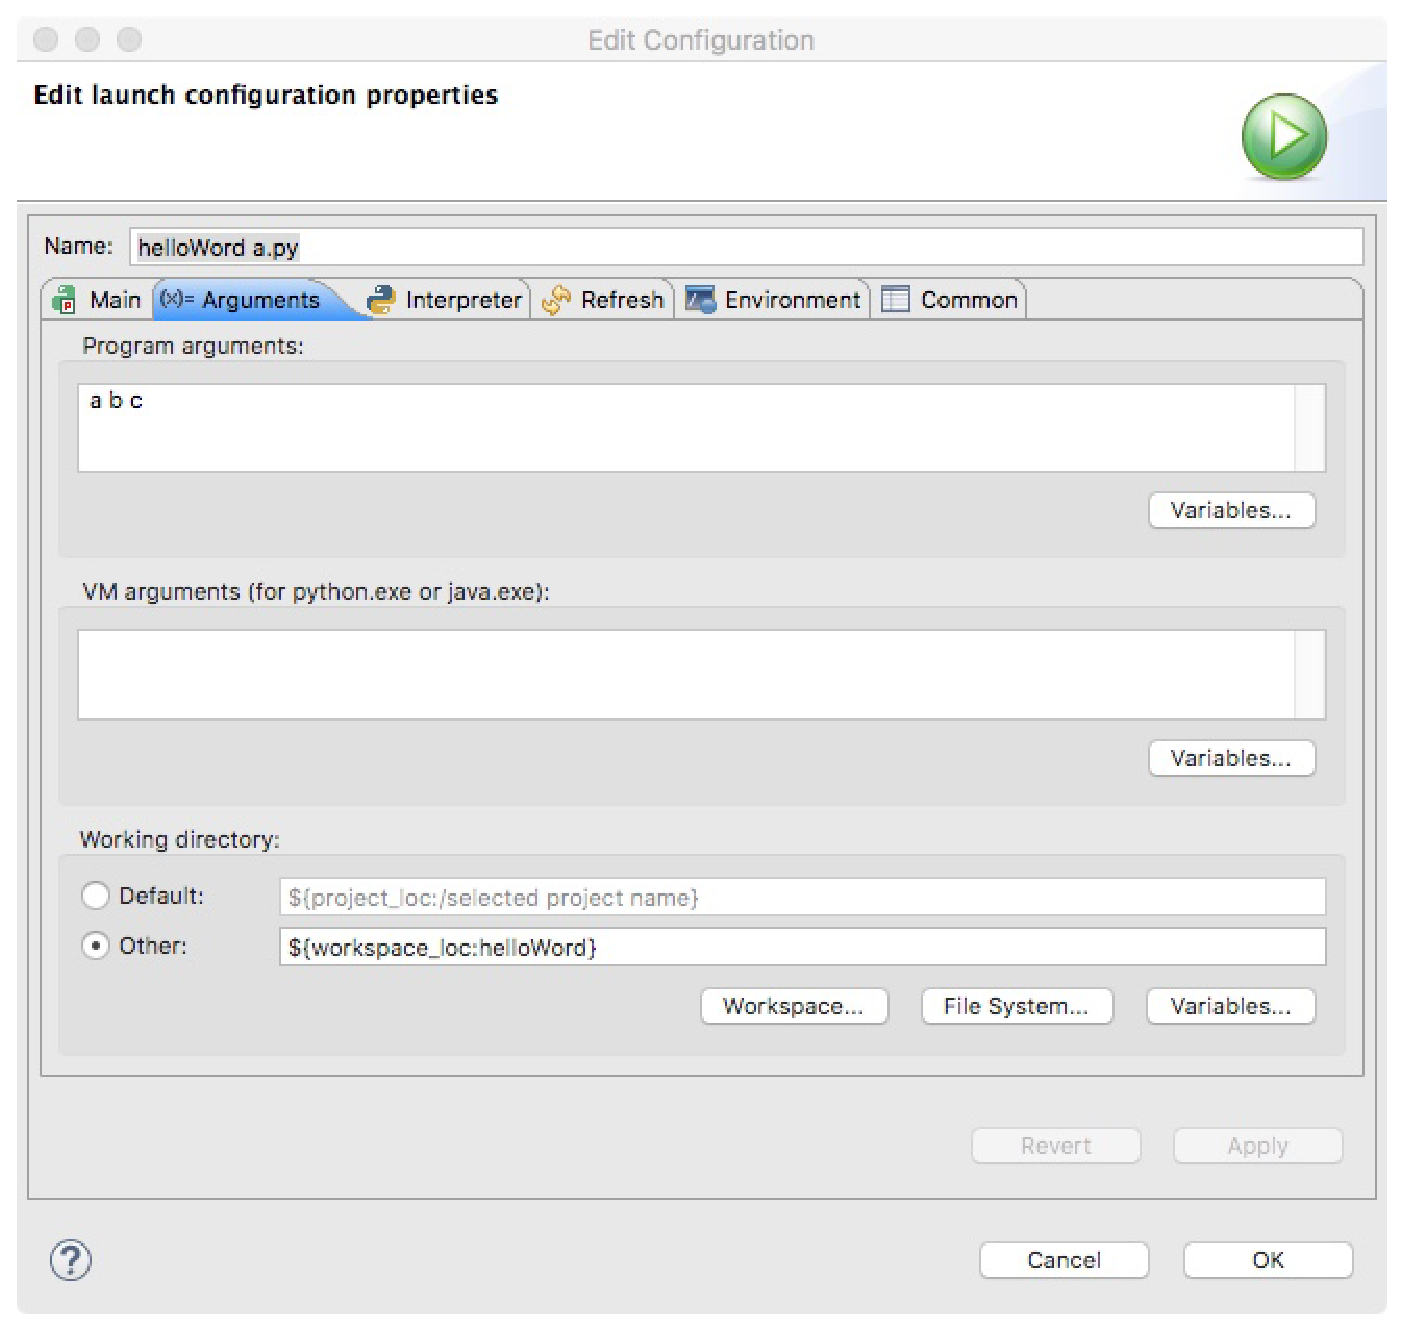
\includegraphics[height=0.65\textwidth]{imagenes/arguments}
\end{center}
\caption{Configuración de argumentos en Eclipse}
\label{fig:argumentos}
\end{figure}

\section{Entrada, salida y errores}

El módulo \texttt{sys}, que hemos usado en el apartado anterior para consultar los argumentos del programa, también nos ofrece tres \emph{flujos} (streams) abiertos para manejar la entrada estándar al programa, la salida estándar y la salida de errores. Se trata de \texttt{sys.stdin}, \texttt{sys.stdout} y \texttt{sys.stderr}. 

Aunque es posible manejar estos flujos de entrada y salida directamente usando las herramientas de lectura y escritura de archivos, en esta sección comentamos el modo de emplearlos indirectamente a través de los métodos \texttt{input()} y \texttt{print()}.

\subsection{Entrada estándar}

El modo más sencillo para leer de la entrada estándar es la función \texttt{input()}, incluida en el propio lenguaje. La función lee una línea completa de la entrada, la convierte a una cadena (eliminando el salto de línea) y la devuelve. Opcionalmente podemos llamar a \texttt{input()} con un argumento que es el \emph{promt} que se mostrará al usuario por salida estándar para invitarle a que escriba:

\begin{lstlisting}
print("Indica tu sketch de los Monty Python favorito")
sketch = input("--> ")
best = ['The Spanish Inquisition','Four Yorkshiremen','Brain Specialist']
if sketch in best:
	print("¡Ése es genial!")
else:
    print("No está mal")
\end{lstlisting}

\subsection{Salida estándar y salida de errores}

Ya hemos visto el uso del método \texttt{print()} en bastantes ejemplos, pero podría indicarse algo más. Hasta ahora, hemos usado \texttt{print()} con uno o varios argumentos separados por comas, y el comportamiento que tiene por defecto consiste en imprimir las cadenas que resultan de invocar a \texttt{str()} sobre cada argumento, dejando un espacio en blanco como separador. Podemos modificar el separador usando el argumento nombrado \texttt{sep}:

\begin{lstlisting}
print('Uno',2,['a','b',3],sep='.+.')
\end{lstlisting}

Un segundo argumento adicional del método \texttt{print()} es \texttt{file}, que permite especificar el flujo a través del cual se va a generar la salida. Por defecto toma el valor \texttt{sys.stdout}, pero podemos usarlo para producir mensajes de error a través de \texttt{sys.stderr}:

\begin{lstlisting}
print('¡Catástrofe: excepción capturada!',file=sys.stderr)
\end{lstlisting}

Los mensajes enviados a la salida de error se muestran en rojo en la consola de Eclipse. Dependiendo del funcionamiento del intérprete de Python, los mensajes de la salida estándar y la salida de error se pueden mezclar. Esto se debe a que los accesos a la consola se intentan reducir para acelerar la ejecución del programa. El texto pendiente de ser emitido por la consola se almacena en un buffer que, llegado el momento que decida el intérprete, se muestra por la salida. Si sólo se usa una salida (normal o de error), no hay problema en la ordenación de los mensajes. Si se emplean las dos, podemos encontrarnos con mezclas extrañas. Para obligar a que se vacíe un flujo en la consola, el método \texttt{print()} tiene otro argumento más: \texttt{flush}. Por defecto toma el valor \texttt{False}, indicando que no hay que imprimir inmediatamente la salida. Si se indica \texttt{True} se fuerza al intérprete a emitir por consola todo lo que tenga almacenado en el buffer asociado al flujo del argumento \texttt{file}.

Otro argumento que puedes usar con el método \texttt{print()} es \texttt{end}. Por defecto, el método genera un salto de línea como último caracter de la cadena que se imprime. Podemos modificar este comportamiento especificando otra cadena en \texttt{end}:

\begin{lstlisting}
print('No imprimas un salto ',end='')
print('porque quiero seguir en la misma línea')
\end{lstlisting}


\section{Ficheros}

Python incluye una función integrada en el propio lenguaje para abrir archivos del sistema: \texttt{open()}. El resultado de la función es una instancia de un tipo de dato que actúa como \emph{descriptor de archivo} y que ya hemos usado con los flujos de entrada estándar, salida estándar y error. Sobre los descriptores de archivo abiertos podremos invocar a una serie de métodos para realizar operaciones de lectura, escritura y cierre de los archivos.

\subsection{Apertura}

El uso más básico del método \texttt{open()} consiste en proporcionarle como argumento el nombre del archivo que queremos abrir. El nombre puede incluir una ruta de directorios delante. Si no la tiene, Python considera que está en el mismo directorio en el que se encuentra el módulo que realiza la apertura. Para usuarios de Windows es importante tener en cuenta que las rutas de archivos usan la contrabarra como separador de directorios. Por esta razón, será conveniente usar el prefijo \texttt{r} en la cadena, de modo que la contrabarra no se interprete como parte de un carácter de escape.

\begin{lstlisting}
archivo = open(r'C:\spam.txt')	
\end{lstlisting}

Por defecto, el modo de apertura es para \emph{lectura}. Y sí, lo has adivinado: si el archivo no existe, excepción al canto. En este caso sería de tipo \texttt{FileNotFoundError}. Por tanto, si no te gusta el riesgo, pon un buen \texttt{try-except} rodeando la apertura del archivo.

Para indicar el modo de apertura, ya sea lectura o escritura, se puede pasar un segundo argumento al método \texttt{open} en forma de cadena de caracteres que tiene el significado siguiente:
\begin{itemize}
	\item \texttt{r}: apertura en modo lectura, que es el modo por defecto. Se lee el fichero desde el comienzo.
	\item \texttt{w}: apertura en modo escritura. Si el fichero existe, lo vacía.
	\item \texttt{a}: apertura en modo escritura. Si el fichero existe, no lo vacía sino que añade lo que se escriba al final del mismo.
	\item \texttt{x}: apertura en modo escritura. Si el fichero existe, salta una excepción \texttt{FileExistsError}.
\end{itemize}

Para abrir un fichero en modo lectura y escritura simultáneamente, hay que añadir el carácter \texttt{+} al modo de apertura. Normalmente se empleará la operación \texttt{seek()} que luego se describe para situar la posición de la seguiente operación de lectura o escritura:
\begin{itemize}
	\item \texttt{r+}: apertura en modo lectura y escritura sin vaciar el fichero. Inicialmente se escribe y lee por el principio.
	\item \texttt{w+}: apertura en modo lectura y escritura, vaciando el fichero si existe.
	\item \texttt{a+}: apertura en modo lectura y escritura. Si el fichero existe, inicialmente se escribe y lee al final del mismo.
	\item \texttt{x+}: apertura en modo lectura y escritura. Si el fichero existe, salta una excepción de tipo \texttt{FileExistsError}.
\end{itemize}

Detras de la indicación del modo de apertura, en la misma cadena, se puede indicar si se quiere manejar el fichero en modo texto o binario:
\begin{itemize}
	\item \texttt{t}: apertura en modo texto, que es el modo por defecto.
	\item \texttt{b}: apertura en modo binario.
\end{itemize}

\begin{lstlisting}
# Apertura en modo lectura/escritura para texto
archivo = open('log.txt','r+t')
\end{lstlisting}

El argumento con el modo de apertura tiene que indicarse en segundo lugar, o bien puede nombrarse con \texttt{mode=}. Un argumento que se nombra con \texttt{encoding} permite especificar cuál es el código de caracteres con el que se debe tratar el archivo. Si no se indica, se manejará el código de caracteres del sistema. Por ejemplo, en Windows se emplea \texttt{cp1252} (una extensión de \texttt{latin1}), pero otros sistemas como Mac OS X o Linux usan \texttt{utf8}:

\begin{lstlisting}
# Apertura en modo escritura con latin1
archivo = open('salida.txt','w',encoding='latin1')
\end{lstlisting}

\subsection{Lectura}

Existen varias posibilidades al leer un archivo con Python: leerlo completamente en una única operación, leerlo línea a línea o leerlo en fragmentos de cierta cantidad de bytes. Vemos por separado cada alternativa.

\subsubsection{Lectura completa}

El modo más sencillo para leer un archivo consiste en invocar al método \texttt{read()} sobre el mismo una única vez:

\begin{lstlisting}
archivo = open('archivo.txt')
contenido = archivo.read()
\end{lstlisting}

En la variable \texttt{contenido} se queda almacenada una cadena con todo el contenido del archivo. Sobre esta cadena se pueden usar los métodos de indexación, troceado o fragmentación que sean necesarios para procesar el contenido.

\subsubsection{Lectura por líneas}

En muchas ocasiones, el procesamiento de un archivo se debe realizar línea a línea. Python nos da tres alternativas para leer una tras otra todas las líneas de un archivo: el método \texttt{readline()} que se invoca sobre el archivo abierto, un iterador sobre el archivo, o bien el método \texttt{readlines()}, que devuelve una lista con todas las líneas del archivo.

El método \texttt{readline()} devuelve sucesivamente las líneas del fichero abierto, incluyendo el salto de línea. Cuando no quedan más líneas, el método devuelve la cadena vacía:

\begin{lstlisting}
archivo = open(nombre)
n = 1
while True:
    línea = archivo.readline()
    if not línea:
        break # Final del archivo
    else:
        print('Línea %d: -%s-' % (n,línea.rstrip()))
        n += 1
\end{lstlisting}

Recuerda que la estructura del \texttt{while} anterior, sólo apta para estómagos fuertes, es una forma de escribir un \emph{do-while} en Python. Una alternativa más elegante para hacer lo mismo consiste en usar un \texttt{for-in} sobre el archivo abierto, que en Python es un objeto sobre el que se puede implementar una iteración:

\begin{lstlisting}
archivo = open(nombre)
n = 1
for línea in archivo:
    print('Línea %d: -%s-' % (n,línea.rstrip()))
    n += 1
\end{lstlisting}

Y vamos con la tercera alternativa: el método \texttt{readlines()}. Mediante este método podemos obtener todas las líneas del archivo en una lista:

\begin{lstlisting}
archivo = open(nombre)
líneas = archivo.readlines()
n = 1
for línea in líneas:
    print('Línea %d: -%s-' % (n,línea.rstrip()))
    n += 1
\end{lstlisting}

Es cuestión de gustos el escoger una u otra.

\subsubsection{Lectura por caracteres o bytes}

Una posibilidad más a la hora de leer los archivos -- especialmente útil cuando se trata de archivos binarios -- es la lectura de bloques de bytes o caracteres. Para ello tenemos que emplear una versión de \texttt{read()} que tiene como argumento el número de bytes o caracteres que se quiere leer:

\begin{lstlisting}
tamaño_cabecera = 10
archivo = open(nombre,"rb")
cabecera = archivo.read(tamaño_cabecera)
for b in cabecera:
	print('%x' % (b), end=' ')
\end{lstlisting}


\subsection{Escritura}

Lo sentimos por los programadores indecisos: también tenemos varias formas de escribir en un fichero. Podemos emplear los métodos \texttt{write()} y \texttt{writelines()} del fichero abierto en modo escritura, o bien podemos usar \texttt{print()} especificando en el parámetro \texttt{file} el fichero.

El método \texttt{write()} es el clásico. Tiene como argumento la cadena que se quiere imprimir, que es una cadena de caracteres en caso de que se haya abierto en modo texto, o bien una cadena binaria si se ha abierto en modo binario:

\begin{lstlisting}
archivo = open('salida.txt','w',encoding='latin1')
archivo.write('De minimis non curat praetor\n')
archivo.write('Aquila non capit muscas\n')
archivo.write('Beati hispani quibus vivere bibere est\n')
\end{lstlisting}

Como alternativa, en caso de que tengamos una lista de cadenas y queramos volcarlas sobre el archivo en el orden en el que se encuentran en la lista, podemos emplear \texttt{writelines()}:

\begin{lstlisting}
archivo = open('salida.txt','w',encoding='latin1')
latinajos = []
latinajos += ['De minimis non curat praetor\n']
latinajos += ['Aquila non capit muscas\n']
latinajos += ['Beati hispani quibus vivere bibere est\n']
archivo.writelines(latinajos)
\end{lstlisting}

Y como tercera alternativa, tenemos el método \texttt{print()} con el argumento \texttt{file}:

\begin{lstlisting}
archivo = open('salida.txt','w')
print('%.2f*%.2f+%.2f=%.2f' % (3.14,2.0,5.1,3.14*2.0+5.1), file=archivo)
\end{lstlisting}

\subsection{Otros métodos}

Para concluir la descripción de las operaciones sobre archivos, comentamos brevemente tres métodos más. En primer lugar, el método de cierre: \texttt{close()}. Como hemos indicado en varias ocasiones, Python emplea un \emph{recolector de basura} para liberar la memoria que ya no se referencia en nuestro programa. Esta recolección incluye a los ficheros abiertos que ya no se pueden usar porque el código ha pasado a otro ámbito y no son alcanzables. Python cierra automáticamente estos archivos antes de liberar los recursos que emplean. Pero nosotros podemos realizar el cierre de forma explícita:

\begin{lstlisting}
archivo.close()
\end{lstlisting}

El cierre lleva a cabo un vaciado del buffer de salida que el intérprete de Python puede estar usando para reducir el acceso al disco. También podemos forzar ese vaciado sin cerrar el archivo, invocando al método \texttt{flush()}:

\begin{lstlisting}
archivo.flush()
\end{lstlisting}

Por último, cuando un archivo se abre en modo lectura y escritura (incluyendo \texttt{+} en el modo de apertura), es muy posible que necesitemos situarnos en diferentes posiciones del archivo en función de la operación que queramos hacer. Sabiendo el desplazamiento \texttt{N} desde el comienzo del fichero, podemos indicar la posición de la siguiente lectura o escritura usando \texttt{seek()}:

\begin{lstlisting}
archivo.seek(N)
\end{lstlisting}


\clearpage{\pagestyle{empty}\cleardoublepage}

% Capítulo 7: Clases
%!TEX root = Python.tex

\chapter{Clases}

\lettrine[lines=5]{V}{amos} a hacer una mínima incursión en el terreno de la programación orientada a objetos con Python. Tiene que ser mínima por dos razones: para aprender el paradigma de programación orientado a objetos ya tenéis la asignatura correspondiente, y no es muy aconsejable mezclar ideas de aquí y allá cuando se está empezando porque la indigestión puede ser importante; y en segundo lugar, si nos metemos a fondo con la orientación a objetos en Python, estos apuntes van a perder su intención inicial de ser pequeños. Por tanto, sólo vamos a contar lo estrictamente necesario y así tendréis la oportunidad de leer con ganas los libros que aparecen indicados en la bibliografía al respecto de esta parte del lenguaje.

\section{Introducción}

Vamos a enfocar el uso de la orientación a objetos como una vuelta de tuerca más de la estructuración del código. Como vimos en el capítulo \ref{chap:modulosPaquetes}, Python está muy preparado para que resulte fácil organizar el código de un proyecto en módulos. Un módulo contiene una serie de definiciones que puedo importar en otro módulo, pero atención, sólo puedo hacerlo una vez. Hasta ahora hemos visto módulos que contienen definiciones de variables y de funciones.

Imagina que quieres hacer un módulo que contenga variables y funciones para representar rectángulos. Aunque se puede hacer, no sería muy estético que con un único módulo, que sólo se puede importar una vez, pudieses representar muchas instancias de rectángulos distintos. Aquí es donde viene en ayuda la definición de clases.

Una clase permite definir un tipo de dato nuevo del cual puedo crear cuantas instancias me apetezca, de modo similar a la forma de crear muchas listas o diccionarios que ya hemos visto. Cada instancia, u \emph{objeto}, tiene su propia memoria, con sus valores de variables, y puedo invocar a métodos sobre cada instancia que trabajen con esos valores y no los de otra instancia.

\subsection{Definición}

Vamos a empezar viendo cómo definir una clase. Dentro de un mismo módulo se pueden crear múltiples clases. Por ejemplo, supongamos que definimos una clase para representar un rectángulo. Podemos hacerlo en un módulo \texttt{figuras2D.py}, dentro del cual definimos la clase empezando con la palabra clave \texttt{class} seguida del nombre de la clase \texttt{Rectángulo}\footnote{Los nombres de clases se escriben comenzando con mayúsculas: \texttt{class DestructorFacultad}. }. Normalmente los nombres de clases se inician con una letra en mayúscula en Python. La clase crea un espacio de nombres nuevo, y todas las definiciones de variables o métodos de la clase se especifican en un bloque indentado a continuación de la línea \texttt{class}. 

\begin{lstlisting}
class Rectángulo:
    # Definición de métodos y variables
\end{lstlisting}

Una clase tiene un primer método especial, porque es el encargado de crear instancias nuevas de la clase. Se llama \emph{inicializador}, y puede recibir argumentos con los valores que permiten definir la nueva instancia. Por ejemplo, un rectángulo se define con el alto y el ancho. El método inicializador siempre se llama igual en Python: \texttt{\_\_init(self,...)\_\_}:

\begin{lstlisting}
class Rectángulo:
    def __init__(self,alto,ancho):
        self.alto = alto
        self.ancho = ancho
\end{lstlisting}

Como ves, además de los argumentos que sirven para definir la instancia nueva, siempre hay un primer argumento en el inicializador y en cualquier otro método de la clase, que se llama \texttt{self}. Se trata de una referencia a la instancia de la clase. En el inicializador, puedo definir variables de las instancias usando la notación \texttt{self.X}, donde \texttt{X} es el nombre de la variable que quiero definir. Normalmente los parámetros que se pasan al inicializador sirven para dar valor a algunas de estas variables. En cualquier método adicional puedo consultar y modificar los valores de estas variables usando \texttt{self.X}.

Podemos añadir un método para calcular el área del rectángulo, siguiendo siempre la convención de poner como primer argumento a \texttt{self}:

\begin{lstlisting}
class Rectángulo:
    def __init__(self,alto,ancho):
        self.alto = alto
        self.ancho = ancho
    def área(self):
        return self.alto*self.ancho
\end{lstlisting}

\subsection{Creación y uso de instancias}

Una vez que hemos definido la clase, podemos probarla con varias instancias y llamadas a sus métodos. Para instanciar un objeto de una clase hay que invocar a su inicializador, usando el nombre de la clase. Una vez que están instanciados los objetos, podemos invocar a métodos sobre cada uno de ellos. Si la clase está en un módulo distinto a aquél que va a usarla, nos hará falta empezar haciendo la importación correspondiente:

\begin{lstlisting}
from figuras2D import Rectángulo
\end{lstlisting}

También podemos probar la clase dentro del módulo \texttt{figuras2D.py}, con algún código de primer nivel que instancie varios objetos e invoque a sus métodos para comprobar que todo va bien:

\begin{lstlisting}
if __name__ == '__main__':
    r1 = Rectángulo(5,4)            # Crea un rectángulo con alto=5 y ancho=4
    r2 = Rectángulo(8.3,20.1)
    print('Area de r1:',r1.área())
    print('Area de r2:',r2.área())
\end{lstlisting}

En muchas ocasiones se crean instancias de una clase dentro de otra clase. Este uso se conoce como \emph{composición} en orientación a objetos.

\subsection{Variables de clase}

Además de definir variables de instancia en el inicializador de la clase, también se pueden definir variables de clase que son compartidas por todas las instancias de la clase. Para ello únicamente hay que definir las variables fuera de los métodos de la clase, sin usar \texttt{self} delante:

\begin{lstlisting}
class Rectángulo:
    tipo = 'rectángulo'   # Variable compartida por todas las instancias
    ...
\end{lstlisting}

\subsection{Visibilidad}

En Python, por defecto, todas las variables y métodos son accesibles para cualquier código que utilice la clase. Existen algunos modos de ocultar las definiciones pero, como se suele decir, queda fuera del ámbito de este documento. Únicamente os recomendamos que sigáis la convención de nombrar con un prefijo de dos guiones bajos \texttt{\_\_X} a los métodos y variables que no queráis que se usen desde fuera de la clase.

\section{Herencia}

Además de la composición, la otra gran ventaja de la orientación a objetos es la \emph{herencia} que consiste en definir clases a partir de otras previamente creadas. La herencia requiere un diseño meditado del código, porque no es algo que se improvise a la ligera. Por ejemplo, si quisiéramos ampliar el módulo \texttt{figuras2D.py} con cuadrados, círculos y demás, nos daríamos cuenta de que todas las clases comparten alguna funcionalidad común, como el método para calcular el área. Podríamos definir una clase base que definiese este método y, mediante herencia, crearíamos los distintos tipos de figuras extendiendo la clase base mediante herencia.

Vamos a ver aplicado el concepto de herencia a una jerarquía de clases que definen puntos en espacios tridimensionales, bidimensionales y unidimensionales. Creamos tres clases \texttt{Punto3D}, \texttt{Punto2D} y \texttt{Punto1D}, y vamos a hacer que la primera de ellas esté en la raíz de la jerarquía de herencia, ya que un punto bidimensional se puede considerar como otro tridimensional en el que la coordenada \texttt{z} es cero; de modo similar, un punto de unidimensional es como uno bidimensional en el que la coordenada \texttt{y} es cero:

\begin{lstlisting}
class Punto3D:
    def __init__(self, x, y, z):
        self.x, self.y, self.z = x, y, z 
    def módulo(self):
        return (self.x**2+self.y**2+self.z**2)**0.5
		
class Punto2D(Punto3D):
    def __init__(self, x, y):
        super().__init__(x, y, 0)

class Punto1D(Punto2D):
    def __init__(self, x):
        super().__init__(x, 0)
		
if __name__ == '__main__':
    p3 = Punto3D(4,2,2)
    p2 = Punto2D(3,4)
    p1 = Punto1D(6)
    print('%.2f %.2f %.2f' % (p3.módulo(),p2.módulo(),p1.módulo()))
\end{lstlisting}

Como vemos en el código anterior, la forma de indicar que una clase hereda de otra consiste en indicar junto al nombre de la clase, entre paréntesis, la clase de la que hereda, también llamada clase \emph{base}. Por ejemplo \texttt{Punto2D(Punto3D)} significa que la clase \texttt{Punto2D} hereda de la clase \texttt{Punto3D}. La herencia implica que todos los métodos y variables de la clase base pasan a ser métodos y variables de la nueva clase, salvo el inicializador. Por ejemplo, el método \texttt{módulo()} se puede invocar también sobre objetos de la clase \texttt{Punto2D}.

En la clase \texttt{Punto2D} se ha definido un inicializador distinto, que sólo tiene argumentos \texttt{x} e \texttt{y}. Desde este inicializador se invoca al de la clase base mediante \texttt{super()}, que permite recuperar una referencia a dicha clase base. Como se puede observar, el argumento \texttt{z} en la invocación de la línea 9 es 0, como corresponde a un punto bidimensional. De forma similar se continúa la jerarquía de herencia a \texttt{Punto1D}.

\section{Comprobaciones con objetos}

Cuando creamos objetos y los guardamos en variables o cualquier tipo de contenedor, lo que estamos haciendo realmente es guardar una referencia a la posición de memoria donde se ha creado el objeto. Python es bueno con nosotros y nos oculta todos los detalles de bajo nivel que en lenguajes más espartanos, como C, tendríamos que manejar nosotros mismos.

Si una variable que contiene una referencia a un objeto se asigna a otra variable, siempre estaremos copiando la referencia, no estaremos creando una copia del objeto en sí. Y recuerda que un objeto puede tener internamente referencias a otros objetos que usa por composición. 

Para comprobar si una referencia que tenemos por un lado apunta al mismo objeto que otra, podemos usar el operador relacional \texttt{is}:

\begin{lstlisting}
p1 = Punto3D(4,2,2)
p2 = p1 # Copiamos referencias
print(p1 is p2) # Imprime True
\end{lstlisting}

Si lo que queremos hacer es comprobar si dos objetos son iguales en el sentido de que contienen exactamente la misma información, aunque sean instancias distintas de una misma clase, podemos usar el operador relacional \texttt{==}:

\begin{lstlisting}
p1 = Punto3D(4,2,2)
p2 = Punto3D(4,2,2)
print(p1 == p2) # Imprime True
print(p1 is p2) # Imprime False
\end{lstlisting}

También podemos comprobar si un objeto es de cierta clase, usando la función \texttt{isinstance()} que ya vimos en la sección \ref{sec:comp_tipos}. Esta función recibe como argumento la referencia al objeto y la clase o tipo. Debido a la herencia, \texttt{isinstance()} devuelve \texttt{True} si comprobamos que un objeto es instancia de toda la jerarquía hasta la clase base:

\begin{lstlisting}
p1 = Punto1D(4)
print(isinstance(p1,Punto1D)) # Imprime True
print(isinstance(p1,Punto2D)) # Imprime True
print(isinstance(p1,Punto3D)) # Imprime True
\end{lstlisting}

Además de las comprobaciones con tipos básicos y clases, \texttt{isinstance()} también permite verificar si una instancia es una lista (\texttt{list}), un diccionario (\texttt{dict}), un conjunto (\texttt{set}) o una tupla (\texttt{tuple}).
\clearpage{\pagestyle{empty}\cleardoublepage}

% Capítulo 8: AFDs en Python
%!TEX root = Python.tex

\chapter{Autómatas en Python}

\lettrine[lines=5]{E}{n} este capítulo iniciamos la descripción de los aspectos que están más relacionados con la asignatura Autómatas y Lenguajes Formales de la FIUM. Concretamente, vamos a centrarnos en el modo de manipular los autómatas finitos deterministas (AFDs) desde el código Python. Los autómatas que podremos manejar tendrán que haber sido editados con la herramienta JFLAP, bien en su versión 7 como en la 8beta. No entraremos en la descripción del formalismo de los AFDs, sino en el funcionamiento del código disponible para usarlos desde Python.

\section{Instalación del paquete \texttt{jflap}}

En los recursos de la asignatura en el Aula Virtual puedes encontrar la carpeta \texttt{Python}. Dentro de ella hay un fichero \texttt{jflap.zip}. Al descomprimirlo se genera una carpeta \texttt{jflap} dentro de la cual encontrarás los siguientes tres ficheros: 

\begin{itemize}
	\item \texttt{\_\_init\_\_.py}: fichero de inicialización del paquete.
	\item \texttt{Afd.py}: es el módulo principal que contiene la clase \texttt{Afd} que manejaremos para manipular el autómata desde Python.
	\item \texttt{Transiciones.py}: es un módulo auxiliar de \texttt{Afd.py}. No es necesario importarlo.
\end{itemize}

Mueve la carpeta \texttt{jflap} al directorio \texttt{src} del proyecto de Eclipse en el que estés trabajando. De los tres ficheros anteriores, únicamente será necesario importar la clase \texttt{Afd} del fichero \texttt{Afd.py}. Para esto, tendremos que usar la siguiente línea de importación desde nuestro código:

\begin{lstlisting}
from jflap.Afd import Afd
\end{lstlisting}

\section{Instanciación de un Afd}

Dependiendo de la versión de JFLAP que estés usando, cambia ligeramente el modo de instanciar un objeto \texttt{Afd}. Puedes ver la versión de JFLAP seleccionando el menú \emph{Help}, opción \emph{About}. Necesitamos dos argumentos:
\begin{itemize}
	\item Ruta del fichero JFLAP que contiene el autómata. Si has usado la versión 7, el fichero tendrá como extensión \texttt{.jff}; si has usado la versión 8beta tendrá como extensión \texttt{.jflap}. Indica la ruta completa, recordando que si estás en Windows conviene que uses \texttt{r'...'} para evitar problemas con las contrabarras que separan los directorios.
	\item Versión del fichero.  La versión del fichero es un número. Debes usar el 6 (sí, no es un error, 6 en lugar de 7) para los ficheros \texttt{.jff} y el 8 para los ficheros \texttt{.jflap}. Si no indicas nada, se usa 6 por defecto.
\end{itemize}

No estaría mal que empleases un \texttt{try-except} similar a éste:

\begin{lstlisting}
from jflap.Afd import Afd
from sys import stderr	
ruta = r'C:\prueba.jff'
try:
    autómata = Afd(ruta)
except FileNotFoundError:
    print('Me temo que la ruta está mal',file=stderr)
except Exception as error:
    print('Problema analizando el fichero:',error,file=stderr)
\end{lstlisting}

La excepción \texttt{FileNotFoundError} se lanza desde el constructor del objeto \texttt{Afd} cuando el fichero pasado como primer argumento no existe. En un programa que solicite el autómata al usuario desde la consola, lo normal sería pedirlo nuevamente. La segunda línea \texttt{except} captura cualquier excepción. Por ejemplo, si el fichero no se puede analizar con la versión especificada como segundo parámetro, se recibirá una excepción que indicará el problema. Igualmente, si la versión especificada no es ni la 6 ni la 8, se lanzará una excepción advirtiéndonos de esto.

En las siguientes secciones consideramos que estamos trabajando con un autómata como el indicado en la figura \ref{fig:prueba_jff}.

\begin{figure}
\begin{center}
\begin{picture}(60,30)(0,0)
\node[Nmarks=i](Q0)(10,15){$q_0$}
\node[Nmarks=r](Q1)(50,15){$q_1$}
\drawedge[curvedepth=8](Q0,Q1){$0$}
\drawloop[loopdiam=6](Q0){$1$}
\drawedge[curvedepth=8](Q1,Q0){$0$}
\drawloop[loopdiam=6](Q1){$1$}
\end{picture}
\end{center}
\caption{Autómata \texttt{prueba.jff}}
\label{fig:prueba_jff}
\end{figure}

\section{Uso de Afd}

En esta sección se proporciona un pequeño manual de uso de un objeto \texttt{Afd}. En primer lugar, veremos cómo imprimir la información del autómata, que nos puede servir en la fase de pruebas. Seguidamente estudiaremos los métodos que son necesarios para simular con el autómata, es decir, para ir recorriendo transiciones desde el estado inicial, usando un símbolo en cada paso.

\subsection{Mostrar el Afd}

Para poder depurar un programa que utiliza un objeto \texttt{Afd}, puede ser interesante imprimir toda la información que contiene para verificar que coincide con el autómata que hemos indicado al instanciar el objeto. Para ello, podemos usar el método \texttt{mostrarAfd()}:

\begin{lstlisting}
autómata = Afd(ruta,versión)
# Depuramos
autómata.mostrarAfd()
\end{lstlisting}

El resultado es un volcado por consola de la información que contiene. Por ejemplo, para el autómata mostrado en la figura \ref{fig:prueba_jff}, veríamos lo siguiente:

\begin{lstlisting}
Número de estados: 2
Número de transiciones: 4
El estado inicial es: 'q0'
Los estados finales son: ['q1']
El alfabeto del autómata es:  ['0', '1']
El estado 'q0' tiene estas transiciones:
{'1' : 'q0', '0' : 'q1' }
El estado 'q1' tiene estas transiciones:
{'0' : 'q0', '1' : 'q1' }
\end{lstlisting}

\subsection{Obtener el estado inicial}

Para validar una cadena con un autómata, necesitamos comenzar el recorrido de los símbolos de la cadena desde el estado inicial. Para recuperar el estado inicial, simplemente tenemos que invocar al método \texttt{getEstadoInicial()} del autómata:

\begin{lstlisting}
autómata = Afd(ruta,versión)
# Inicio de la simulación
estadoActual = autómata.getEstadoInicial()
print(estadoActual)
\end{lstlisting}

\subsection{Consultar una transición}

Supongamos que disponemos de una variable \texttt{simboloActual} que contiene el siguiente símbolo a procesar de la cadena. Necesitaremos comprobar si, desde el estado actual, se puede avanzar a un nuevo estado recorriendo alguna transición con el símbolo actual. Disponemos del método \texttt{estadoSiguiente()} para realizar esta consulta:

\begin{lstlisting}
estadoSig = autómata.estadoSiguiente(estadoActual,simboloActual)
print(estadoSig)
\end{lstlisting}

Este método recibe como argumentos el estado actual y el símbolo actual, y devuelve el estado al que se llega o \texttt{None} en caso de que la transición no esté definida.

\subsection{Comprobar si un estado es final}

Para verificar si una cadena se valida, debemos comprobar si el último estado al que se llega tras recorrer todos sus símbolos es final. Para realizar esta comprobación disponemos del método \texttt{esFinal()}:

\begin{lstlisting}
estadoSig = autómata.estadoSiguiente(estadoActual,simboloActual)
print(autómata.esFinal(estadoSig))
\end{lstlisting}

Devuelve \texttt{True} en caso de que sí lo sea, \texttt{False} en caso contrario.

\subsection{Obtener el alfabeto del autómata}

Se puede consultar el alfabeto que emplea el autómata con el método \texttt{getAlfabeto()}:
\begin{lstlisting}
# Conjunto de símbolos
alfabeto = autómata.getAlfabeto()
\end{lstlisting}
\clearpage{\pagestyle{empty}\cleardoublepage}

% Capítulo 9: Expresiones regulares
%!TEX root = Python.tex

\chapter{Expresiones regulares}

\lettrine[lines=5]{M}{uchas} de las aplicaciones que aprovechan de forma práctica los principios teóricos de la asignatura Autómatas y Lenguajes Formales, emplean \emph{expresiones regulares} (ER) para la validación, búsqueda y sustitución de cadenas de caracteres. La validación la podemos encontrar en cualquier aplicación que reciba una entrada que puede contener errores de formato, como los campos de un formulario rellenados por una persona; un DNI o un código bancario IBAN tienen una estructura perfectamente definida que se debe verificar antes de aceptar la entrada del usuario. Las búsquedas forman parte de infinidad de aplicaciones, como los procesadores de texto, las herramientas de consulta de bases de datos o los \emph{spiders} que recorren la web o las redes sociales y extraen información que aparece en determinados campos de páginas HTML o contenidos XML. Por último, las operaciones de sustitución son la base para la construcción de traductores, es decir, programas que reciben una entrada en un determinado formato y generan la salida en otro formato. La interconexión de muchas aplicaciones desarrolladas por empresas distintas sería imposible sin estas traducciones entre distintos formatos.

En este capítulo analizamos cómo emplear las expresiones regulares extendidas en Python con la finalidad de realizar las tres operaciones indicadas anteriormente. Como complemento a este capítulo, conviene que tengas a mano el documento que puedes encontrar en el Aula Virtual \texttt{Tutorial\_sintaxis\_ER.pdf}.

\section{Paquetes \texttt{re} y \texttt{regex}}

Toda la funcionalidad de Python relativa a expresiones regulares se encuentra en uno de los paquetes estándares de la distribución de Python, llamado \texttt{re}. Vaya por adelantado la dirección en la que puedes resolver todas las dudas que se te ocurran, y más, sobre el funcionamiento de este paquete: \url{https://docs.python.org/3/library/re.html}. 

Sin embargo, el paquete \texttt{re} no tiene soporte para expresiones regulares del tipo \texttt{$\backslash$p\{L\}}. Por esta razón, conviene que instalemos el paquete \texttt{regex} mediante la herramienta \texttt{pip} en nuestro sistema:

\begin{lstlisting}
pip install regex
\end{lstlisting}

Todos los métodos definidos en el paquete \texttt{re} están en \texttt{regex}, ampliando el soporte de expresiones regulares. Puedes hacer así la importación del paquete \texttt{regex}:

\begin{lstlisting}
import regex as re
\end{lstlisting}

Y puedes encontrar informacion sobre \texttt{regex} aquí: \url{https://pypi.org/project/regex/}.

\subsection{Representación de la expresión regular}

En primer lugar, y a riesgo de ser pesados, conviene recordaros que las expresiones regulares hay que representarlas en Python con cadenas \emph{raw}, ya que es habitual usar contrabarras en la notación de expresiones regulares extendida:

\begin{lstlisting}
patrón_dni = r'\d{8}[A-Z]' # Patrón para DNI
\end{lstlisting}

\subsection{Compilación de la expresión regular}

Antes de usar una expresión regular conviene compilarla. El proceso de compilación implica el análisis de la expresión regular y su conversión a un autómata finito. Como es un proceso costoso, especialmente en el caso de expresiones regulares complejas, hay que evitar en la medida de lo posible la repetición de la operación de compilación de una misma expresión regular:

\begin{lstlisting}
patrón_dni = r'\d{8}[A-Z]' # Patrón para DNI
er_dni = re.compile(patrón_dni) # Objeto ER
\end{lstlisting}

\subsection{Validación de cadenas}

Para comprobar que una cadena completa se valida con una expresión regular, disponemos del método \texttt{fullmatch()} que podemos invocar sobre el objeto ER previamente compilado:

\begin{lstlisting}
import regex as re

if __name__ == '__main__':
    patrón_dni = r'\d{8}[A-Z]' # Patrón para DNI
    er_dni = re.compile(patrón_dni) # Objeto ER
    cadena = input('Introduce un DNI: ')
    result = er_dni.fullmatch(cadena.rstrip())
    if result:
        print('Cadena validada')
    else:
        print('Cadena rechazada')
\end{lstlisting}

El resultado del método \texttt{fullmatch()} es \texttt{None} en caso de que la cadena no se valide, y en caso de que sí se valide es un objeto \texttt{Match}. La utilidad de este objeto la veremos inmediatamente con otros métodos. En el caso de \texttt{fullmatch()}, al hacer una comprobación sí/no, únicamente sirve a modo de resultado booleano.

Python incluye un segundo método de validación de cadenas algo más laxo que \texttt{fullmatch()}: el método \texttt{match()} valida si algún prefijo de la cadena proporcionada como argumento verifica el patrón de la ER. En el ejemplo anterior, si introducimos \texttt{12345678ALF}, también se devuelve un objeto \texttt{Match}. En este caso, podemos saber el prefijo que ha verificado la ER usando los métodos \texttt{start()} y \texttt{end()} del objeto \texttt{Match} devuelto:

\begin{lstlisting}
result = er_dni.match(cadena.rstrip())
if result:
    print('Validado',cadena[result.start():result.end()])
\end{lstlisting}

Opcionalmente, los métodos \texttt{fullmatch()} y \texttt{match()} pueden tener otros dos parámetros más para indicar desde qué posición de inicio y hasta qué posición de final de la cadena se debe hacer la verificación:

\begin{lstlisting}
er_digitos = re.compile(r'\d+')
result = er_digitos.fullmatch('abc123def',3,6)
\end{lstlisting}


\subsection{Búsqueda de cadenas}

Tratamos a continuación dos formas de buscar subcadenas que cumplen un determinado patrón dentro de una cadena mayor. 

Si sólo nos interesa encontrar la primera aparición de la subcadena, se puede emplear el método \texttt{search()} sobre la expresión regular compilada. Este método recibe como argumento la cadena en la que se busca y devuelve un objeto \emph{match} en caso de que se haya encontrado una aparición del patrón, o \texttt{None} en caso de que no aparezca:

\begin{lstlisting}
er_digitos = re.compile(r'\d+')
n = 1
cadena = 'AB 12 DE 34'
m = er_digitos.search(cadena)
if m:
	print('Resultado %d: %s' % (n,cadena[r.start():r.end()]))
else:
	print('No encontrado')
\end{lstlisting}

Para localizar las subcadenas no solapadas que cumplen un determinado patrón dentro de una cadena mayor, haciendo un recorrido de izquierda a derecha de la misma, lo más conveniente es usar un iterador que podemos obtener con el método \texttt{finditer()}:

\begin{lstlisting}
er_digitos = re.compile(r'\d+')
n = 1
cadena = 'AB 12 DE 34'
for r in er_digitos.finditer(cadena):
	print('Resultado %d: %s' % (n,cadena[r.start():r.end()]))
	n += 1
\end{lstlisting}

El iterador asigna a la variable indicada en el \texttt{for} un objeto \texttt{Match}. Al igual que con los métodos \texttt{fullmatch()} y \texttt{match()}, los métodos \texttt{search()} y \texttt{finditer()} pueden tener dos parámetros opcionales para indicar la posición de inicio y fin de la búsqueda.

\subsection{Sustituciones}

Otra operación común que se puede implementar fácilmente con la ayuda de las expresiones regulares es la búsqueda y sustitución de cadenas. En Python se puede usar el método \texttt{sub()} para esta operación. El primer argumento es la cadena de remplazo que sustituye a las ocurrencias de la ER; el segundo argumento es la cadena sobre la que se realiza la búsqueda y sustitución; un tercer argumento permite indicar el número máximo de sustituciones (si no se indica, no hay número máximo). El resultado de la llamada a \texttt{sub()} es la cadena con las sustituciones ya realizadas:

\begin{lstlisting}
er_digitos = re.compile(r'\d+')
cadena = 'AB 12 DE 34'
nueva = er_digitos.sub('-',cadena)
print(nueva) # Imprime 'AB - DE -'
\end{lstlisting}

Si no es posible realizar ninguna sustitución, se devuelve la misma cadena que se pasó como segundo argumento.

Una posibilidad bastante útil del método \texttt{sub()} consiste en que el primer argumento, en lugar de ser una cadena estática, sea el nombre de un método. Este método recibirá como argumento un objeto \texttt{Match} correspondiente a la coincidencia previa a la sustitución, y debe devolver la cadena que lo sustituye. Por ejemplo:

\begin{lstlisting}
def sust(m):
    suma = 0
    for i in m.group(0):
        suma += int(i)
    return str(suma) 

if __name__ == '__main__':
    er_digitos = re.compile(r'\d+')
    cadena = 'AB 12 DE 34'
    nueva = er_digitos.sub(sust,cadena)
    print(nueva) # Imprime 'AB 3 DE 7'
\end{lstlisting}

El método \texttt{sust()} llama al método \texttt{group(0)} el objeto Match para recuperar la cadena que se va a sustituir. En la siguiente sección se trata en detalle el uso de grupos.

\section{Grupos}

Una expresión regular puede definir grupos usando paréntesis. Por ejemplo:

\begin{lstlisting}
patrón_dni = r'(\d{8})([A-Z])' # Patrón para DNI con dos grupos
\end{lstlisting}

La expresión regular anterior define dos grupos, o lo que es lo mismo, dos fragmentos de la expresión regular global indicados entre paréntesis: los dígitos del DNI forman el primer grupo, y la letra mayúscula forma el segundo grupo. Cualquiera de las operaciones vistas en la sección anterior, de validación, búsqueda y sustitución, puede aprovechar el uso de los grupos. 

\subsection{Grupos en validación y búsqueda}

En el caso de las operaciones de validación y búsqueda, podemos extraer la porción de la cadena de entrada que se ha reconocido con cada grupo mediante el objeto \texttt{Match} devuelto por la operación, y el método \texttt{group()} del mismo. Este método recibe como argumento un entero. Si es 0, el método devuelve la cadena completa reconocida con toda la expresión regular. Si es 1, devuelve la porción reconocida a través del primer grupo, y así sucesivamente:

\begin{lstlisting}
patrón_dni = r'(\d{8})([A-Z])' # Patrón para DNI con dos grupos
er_dni = re.compile(patrón_dni) # Objeto ER
cadena = input('Introduce un DNI: ')
result = er_dni.fullmatch(cadena.rstrip())
if result:
    print('DNI',result.group(0),'validado')
    print('Dígitos:',result.group(1))
    print('Letras:',result.group(2))
\end{lstlisting}

Dependiendo de la expresión regular, no todos los grupos pueden haber sido usados en la validación de la cadena. En caso de que un grupo no se use durante la validación, el método \texttt{group()} devuelve \texttt{None}. Por ejemplo:

\begin{lstlisting}
patrón = r'(\d+)|(\p{L}+)|([ \r\t\n]+)'
er = re.compile(patrón)
cadena = 'AB 12 DE 34'
for r in er.finditer(cadena):
    if r.group(1):
        print('Dígitos',r.group(1))
    elif r.group(2):
        print('Letras',r.group(2))
    else:
        print('Espacios en blanco')
\end{lstlisting}

Como alternativa al método \texttt{group()} se puede usar el objeto \texttt{Match} con indexación:

\begin{lstlisting}
patrón = r'(\d+)|(\p{L}+)|([ \r\t\n]+)'
er = re.compile(patrón)
cadena = 'AB 12 DE 34'
for r in er.finditer(cadena):
    if r[1]:
        print('Dígitos',r.group(1))
    elif r[2]:
        print('Letras',r.group(2))
    else:
        print('Espacios en blanco')
\end{lstlisting}

\subsection{Grupos en sustituciones}

Las cadenas de remplazo usadas en las sustituciones pueden usar la información de los grupos obtenida en la operación de búsqueda previa al remplazo. La subcadena reconocida a través del grupo \texttt{N} se puede referenciar desde la cadena de remplazo mediante \texttt{$\backslash$N}:

\begin{lstlisting}
er_digitos = re.compile(r'[A-Z]{2}(\d+)')
cadena = 'AB12 DE34'
nueva = er_digitos.sub(r'-\1-',cadena)
print(nueva) # Imprime '-12- -34-'
\end{lstlisting}

\subsection{Otras formas de referenciar grupos}

Si una expresión regular es muy extensa, es posible que necesitemos usar paréntesis no sólo para denotar grupos, sino simplemente para agrupar partes de la expresión regular con el fin de que los operadores de la misma se combinen como nosotros queramos. Puede llegar a ser una auténtica pesadilla ir contando los paréntesis para ver cuáles representan un grupo y cuáles no. 

Una primera forma de simplificar el problema consiste en marcar de una forma especial los paréntesis que \emph{no} denotan un grupo. Esto se consigue usando la notación \texttt{(?:...)}, es decir, añadiendo \texttt{?:} detrás del paréntesis de apertura. Estos paréntesis no cuentan a la hora de enumerar los grupos:

\begin{lstlisting}
patrón = r'((?:a|b|c)+)|(\d+)'
er = re.compile(patrón)
cadena = 'aaba12ab'
for r in er.finditer(cadena):
    if r.group(1):
        print('Letras:'+r.group(1))
    elif r.group(2):
        print('Números:'+r.group(2))
\end{lstlisting}

Una segunda forma de abordar el uso de grupos consiste en darles un nombre, en lugar de un número que depende del orden de apertura y cierre de paréntesis. Los nombres se indican con la notación \texttt{(?P<nombre>...)}. El método \texttt{group()} del objeto \texttt{Matcher} puede recibir como argumento el nombre del grupo que queremos recuperar:

\begin{lstlisting}
patrón_dni = r'(?P<digitos>\d{8})(?P<letra>[A-Z])' 
er_dni = re.compile(patrón_dni) # Objeto ER
cadena = input('Introduce un DNI: ')
result = er_dni.fullmatch(cadena.rstrip())
if result:
    print('DNI',result.group(0),'validado')
    print('Dígitos:',result.group('digitos'))
    print('Letras:',result.group('letra'))
\end{lstlisting}

En las cadenas de sustitución podemos usar \texttt{$\backslash$g<nombre>} como referencia a un grupo nombrado en la expresión regular.

\clearpage{\pagestyle{empty}\cleardoublepage}

% Capítulo 10: Documentación del código
%!TEX root = Python.tex

\chapter{Documentación de Python}

\lettrine[lines=5]{F}{inalizamos} estos apuntes de Python con una explicación breve sobre el modo habitual de documentar el código. Si vas hacia atrás unas cuantas hojas, y más concretamente a la sección \ref{sec:comentarios} en la que tratábamos los comentarios de código en Python, podrás ver que el esqueleto que generó Eclipse para \texttt{helloword.py} incluía al comienzo una cadena de múltiples líneas que comenzaba y terminaba con tres comillas. Este tipo de cadena se conoce como \emph{docstring}. Hay ciertas partes del código de Python en las que podemos introducir estas cadenas para documentar lo que estamos haciendo. Por supuesto, a nadie le gusta documentar el código. ¡Que el que lo lea se esfuerce en entenderlo! Pero cuando te toca a ti darle vueltas a lo que ha escrito otro, no viene nada mal algunas palabritas sobre lo que ha hecho. 

En el código Python, al menos, deberíamos describir los módulos, las clases y las funciones. La documentación del módulo debe aparecer justo al comienzo del fichero, mientras que la de una clase o un método se indica justo a continuación de la línea \texttt{class} o la línea \texttt{def}. El esquema de la documentación es el siguiente:

\begin{lstlisting}
'''
Documentación del módulo
'''

class X:
    '''
    Documentación de la clase
    '''

    def metodo(args):
        '''
        Documentación de la función
        '''
\end{lstlisting}

En la siguiente sección indicamos sugerencias sobre lo que puede especificarse en cada cadena de documentación. No vamos a usar ningún sistema complejo para documentar el código, del estilo de \emph{reStructured}. Ten en cuenta que en esta asignatura no tienes que entregar una memoria de prácticas. A cambio, los profesores de la asignatura evaluamos que seas generoso en la documentación del código.

\section{Formato de la documentación}

La documentación de módulos, clases y funciones sigue un formato muy libre. Se realiza con cadenas multilínea (con tres comillas simples o dobles), y se recomienda que tenga las siguientes partes:
\begin{enumerate}
	\item Tras la apertura de la cadena, escribimos una línea en forma de resumen o título.
	\item Dejamos una línea en blanco después del resumen.
	\item A continuación escribimos una serie de líneas adicionales en las que nos podemos extender lo que queramos, evitando superar los 72 caracteres por línea.
	\item Después del cierre de la cadena, se deja una línea en blanco antes del código que viene a continuación.
\end{enumerate}

\subsection{Documentación de una clase}

Cuando describimos una clase, al menos deberíamos indicar lo siguiente:
\begin{itemize}
	\item Un breve resumen del propósito de la clase.
	\item Un listado de los atributos (de clase o instancia).
	\item Un listado de los métodos que queremos que se usen desde el código cliente.
\end{itemize}

Por ejemplo:

\begin{lstlisting}
class Afd:
    '''
    Clase que representa un fichero JFLAP en Python
	
    Atributos
    ---------
    nestados: int 
        Número de estados del autómata
    ntransiciones: int
        Número de transiciones del autómata

    Métodos
    -------
    getEstadoInicial() : str
        Devuelve el nombre del estado inicial
    esFinal(estado : str) : bool
        Devuelve True si el estado es final
    estadoSiguiente(estado : str, símbolo : str) : str
        Devuelve el destino de una transición
    '''
\end{lstlisting}

\subsection{Documentación de un método}

La documentación de los métodos puede ser más explícita a la hora de describir lo que estos hacen. Por ejemplo, se puede indicar:
\begin{itemize}
	\item Una breve descripción de lo que hace el método y cómo se usa.
	\item Una descripción de los argumentos, tanto requeridos como opcionales o nombrados.
	\item En el caso de los atributos opcionales, el valor por defecto que toman.
	\item Una descripción de cualquier excepción que se puede lanzar desde el método y en qué circunstancias.
\end{itemize}

Este podría ser un ejemplo:
\begin{lstlisting}
def estadoSiguiente(self, estado, símbolo)
    '''
    Devuelve un str con el destino de una transición desde un estado
    y con un símbolo dados. Si no existe una transición con esas 
    características, devuelve None.
	
    Parámetros
    ----------
    estado: str
        Estado desde el que se inicia la transición
    símbolo: str
        Símbolo que etiqueta la transición
\end{lstlisting}

\subsection{Documentación de un módulo}

En la parte superior de un módulo es conveniente escribir una descripción general del mismo que puede contener, entre otras cosas, lo siguiente:
\begin{itemize}
	\item Título del módulo y fecha de creación.
	\item Autor indicado tras \texttt{@author:}.
	\item Descripción general de las clases o métodos agrupados en el módulo y su funcionalidad común.
	\item Indicación de las dependencias del módulo, como los paquetes que deben estar instalados para poder usarlo.
	\item Indicación de la funcionalidad del módulo a través del código de primer nivel, en caso de que tenga un punto de entrada \texttt{\_\_main\_\_}.
\end{itemize}

\section{Uso de la documentación}

Al margen de permitir al que lee el código fuente una comprensión mayor sobre lo que realiza, podemos usar alguna herramienta que saca provecho de los \emph{docstrings} que hemos introducido en el código. Una de ellas es \texttt{help}. Desde el intérprete interactivo de Python podemos importar un módulo y consultar su documentación usando dicho comando. Por ejemplo:

\begin{lstlisting}
>>> import jflap.Afd
>>> help(jflap.Afd)
\end{lstlisting}

\clearpage{\pagestyle{empty}\cleardoublepage}

\bibliography{bibliografia}
\addcontentsline{toc}{chapter}{Bibliografía}
\bibliographystyle{unsrt}

\clearpage{\pagestyle{empty}\cleardoublepage}

\end{document}